% Much of these are still open because I haven't leveraged more recent (i.e. better) data.  So worth re-doing the analysis with it (I have better data & I'm better at coding & after writing this I see how it all fits together).

% Does it make sense to introduce methods (plus investigations, specifically for ACF/XCF) BEFORE describing the whole 'pipeline'?  This chapter is getting unwieldy, especially when I go back and forth between the mathematical methods.
\chapter{Analysis of oscillatory time series}
\label{ch:analysis}

% Introduction: overview of the 'pipeline'
\section{Overview}
\label{sec:analysis-overview}

% - Zielinski et al. (2014) is a good starting point

% From synthetic oscillations report
In the time series analysis literature, there is a wealth of analysis methods that aim to find parameters pertaining to the periodicity of noisy time series and that aim to characterise the relationship between two signals.
This is relevant for biological time series, especially because they are noisy due to both intrinsic and extrinsic noise sources, and because researchers often record multiple time series from the same system to study the relationship between such time series.
One example is the yeast metabolic cycle, which is known to be a metabolic oscillator that is coupled with the cell division cycle oscillator -- in this case, the two time series from this system consist of the level of metabolites to represent the metabolic oscillator and the activity of a component of the cell division cycle to represent the cell division cycle.

The problem with applying classical time series analysis methods to biological time series lies with two properties of biological time series: they are noisy and they are often short.
Classical methods such as Fourier analysis have been shown to be useful in characterising noisy biological time series when they are long, e.g. from neuron impulse recordings, which can include up to thousands of oscillations.
However, for examples such as the yeast metabolic cycle, it is not feasible to record time series that include such a high number of oscillations; in this case, 5-10 oscillations are more realistic.
As a result, methods like Fourier analysis only provide poor resolution for characteristics such as the period of oscillations.
% ----- end from synthetic oscillations report

To discuss the process of analysing oscillatory time series in more detail, I will be using my data as an example and divide this chapter according to steps in the process.
My data consists of 100--1000 time series of recorded flavin intensity changes for each cell, indicating the yeast metabolic cycle.
Some experiments include HTB2::mCherry strain cells, and I obtain both flavin intensity changes and mCherry intensity changes from each cell;
the mCherry indicating the cell division cycle.
In these time series, there is a new time point every 5 minutes, for a total of 100--300 time points.
These data are stored as dataframes for each condition (strain and media conditions), with the time series as rows and time points as columns --
in the case of HTB2::mCherry cells, the flavin and mCherry time series are in separate dataframes.

This chapter is divided into six sections, five of which correspond to a process and questions each process address:
\begin{enumerate}
  \item Cleaning: choosing data, filtering confounding trends, dealing with missing time points.
  \item Classification: is my time series oscillatory?
  \item Characterisation: I have one time series -- what properties does it have?
  \item Clustering: I have many time series (of the same signal) from many cells -- what are their relationships to each other?
  \item Correlation: I have two signals from the same cell -- what are their relationships to each other?
  \item Summary: bringing it all together in a pipeline.
\end{enumerate}

\section{Cleaning: choosing data, filtering, missing time points}
\label{sec:analysis-cleaning}

The first step of any data science pipeline is cleaning data, and of course there is the adage: 80\% of data science is cleaning data [CITATION NEEDED].
Cleaning data is important because of the principle of `garbage in, garbage out' -- regardless of how cutting-edge the analysis methods are, if the input data is flawed, then you cannot get good insights from the data.
However, this step involves the most judgement calls, i.e. the analyst needs to decide on criteria to separate useful data from useless data.
These criteria may be based on existing standards of practice or, for systems biology, knowledge of either the underlying biological processes or of the mathematical constraints.
Often, these criteria can be arbitrary because there is an absence of existing standards of practice for the specific situation -- in this case, any decision is going to be a trade-off and needs justification.

Three problems I occur in my data are: choosing data, time series filtering, and dealing with missing time points.
They can best be illustrated in a heatmap of raw data from an experiment [DESCRIBE THE EXAMPLE EXPERIMENT] here:

[FIGURE: A HEATMAP BASED ON RAW DATA.  IT SHOULD CONTAIN SOME TRACES THAT DON'T FILL 80\% OF THE TIME COURSE -- SOME EXAMPLE ROWS SHOULD BE LABELLED  IT SHOULD CLEARLY SHOW A LONG-TERM TREND.  IT MAY HAVE MISSING TIME POINTS BECAUSE OF THE LIMITATIONS OF MERGER.  THE CAPTION MUST DESCRIBE THE COMPONENTS OF THE HEATMAP SO A READER CAN INTERPRET IT -- E.G. AXES, COLOUR SCHEME]

[THIS FIGURE MAY HAVE SOME AUXILLARY FIGURES TO HELP EXPLAIN.  I CAN PICK ONE TIME SERIES OUT OF THE HEATMAP, REPRESENT IT AS A LINE PLOT, HIGHLIGHT THE FIRST COUPLE OF TIME POINTS, AND HAVE BRIGHTFIELD AND FLAVIN IMAGES THAT CORRESPOND TO THESE TIME POINTS.  USE ImageViewer TO PRODUCE THIS FIGURE.  I SHOULD HAVE EXPLAINED ENOUGH IN THE METHODS TO HAVE THIS MAKE SENSE.]

The first step is choosing data.
Some time series have few time points.
Most often, these correspond to cells that were not present in traps for a long duration, and some can be the result of errors in the track merging algorithm used in the data extraction process [CAN I CITE ALAN'S THESIS?].
Here, I choose time series that have points present in at least 80\% of the total time points.
This is an arbitrary cut-off, but it ensures that my time series have enough oscillations for further analysis, such as characterisation of the frequencies of these oscillations.
Otherwise, short, and likely uninformative, time series can `pollute' algorithms that operate on the population of time series, confounding the analysis.

Next, the data must be filtered to remove long-term trends.
Depending on the scientific question, such long-term trends can be useful:
for example, in climate science, if there is a time series of atmospheric \ce{CO2} over a period of decades, we would like to filter out the annual (seasonal) cycles and look at the long-term changes over time.
In the analysis of biological rhythms, however, long-term trends are the element that must be removed to uncover the periodic behaviour of biological time series \parencite{zielinskiStrengthsLimitationsPeriod2014} [OR IS THE 2022 PUBLICATION BETTER SUITED TO PROVE MY POINT?  IN ANY CASE, LIFT A COUPLE SENTENCES FROM THEIR DISCUSSION OF REMOVING TRENDS IN BIOLOGICAL TIME SERIES DATA].
As an example, \textcite{zielinskiPeriodEstimationRhythm2022} offers several methods of detrending time series: polynomial detrending (including linear detrending), sliding-window detrending, ... [READ THE PAPER AND INSERT THE REST HERE].
However, each method has its own caveats.

[FIGURE: SHOW LONG-TERM TRENDS.  DRAW A MEAN+STD ERR PLUS A COUPLE OF RAW TIME SERIES.]

In the process of finding a way to filter my time series, I have considered two methods: sliding-window methods (such as using a Savitzky-Golay filter) and a high/low-pass filter.
Sliding-window methods are common in the single-cell biological rhythm literature; for example... [EITHER (A) VOMIT A LIST OF CITATIONS AND LEAVE IT THERE, OR (B) MENTION A COUPLE AND DESCRIBE IN A BIT MORE DETAIL, GROUP SAVITZKY-GOLAY FILTERS, PUBLICATIONS THAT USE STUPIDER METHODS, ETC.  I'M SURE HEINEMANN'S PUBLICATIONS USE THEM, AND I'M SURE THERE WERE A COUPLE USED IN JOURNAL CLUBS THAT I'VE COMMENTED IN MY NOTES HAVING USED STUPID METHODS.]
However, these methods unnecessarily smooth data, therefore distorting the data and affecting conclusions, and give no control over the frequencies and introduce artefacts in the frequency spectrum (figure ...)
In contrast, defining a high- or low-pass filter offers direct control over frequencies, but the user must use a judgement call to define a critical frequency.
In my case, I define the critical frequency for a high-pass filter as 1/350 min-1 [PROPERLY FORMAT UNITS PLEASE] as this corresponds to the upper limit of reasonable durations of yeast metabolic cycles and cell division cycles that I have observed in my single-cell microfluidics experiments.
Of course, this will exclude the possibility of metabolic cycles that go on for longer, but as I said, this is a trade-off I am willing to make so that I can extract the individual oscillations better.

[FIGURE: SHOW HOW SLIDING WINDOW AND HIGH-PASS FILTER AFFECT TIME SERIES DIFFERENTLY.  SHOW RAW TIME SERIES AND FFT, AND SHOW PROCESSED TIME SERIES AND FFTS.  FOR HIGH-PASS FILTER, ALSO DRAW A VERTICAL LINE TO SHOW THE CRITICAL FREQUENCY ON THE FFT.  ALSO ADD A FIGURE SIMILAR TO THE ONE IN THE scipy DOCUMENTATION ON THE HIGH-PASS FILTER TO SHOW THAT THE RELEVANT FREQUENCIES HAVE BEEN DESTROYED.]

Next, missing time points can pose a problem, especially when many analysis methods [WHICH?] are not made for this.
In my case, these missing time points often arise because of errors in track joining [MORE ELABORATION PLEASE -- READ ALAN'S THESIS], but occur infrequently enough [EVIDENCE NEEDED] that I could just perform linear interpolation to fill in the data or discard the time series altogether.
However, there are methods that deal with missing time points.
Most notable is the Lomb-Scargle periodogram (LSP) -- to be discussed in section ... -- which was developed for astronomical data that often has missing time points, corresponding to cloud cover, for example.
Other methods that have been used in the biological time series literature include ... [FISH OUT SOME FROM ZIELINSKI ET AL. 2014, AND DESCRIBE THEM A BIT].

Finally, I discuss a way to evaluate the quality of a (processed) dataset -- specifically, computing a signal-to-noise ratio.
[PROBABLY MAKES SENSE TO DO A MINI-LITERATURE REVIEW OF THE SIGNAL-TO-NOISE RATIO CONCEPT, ESPECIALLY IN THE CONTEXT OF ENGINEERING].
Here, I define a cut-off frequency between signal and noise, based on the assumption that very high-frequency components of the periodogram correspond to noise and lower-frequency components correspond to the meaningful oscillations (and this is after filtering out the very low-frequency components that are the long-term trends I don't want).
[I BASED THIS OFF A POST ON STACKOVERFLOW -- ONE OF THE GIT COMMIT MESSAGES HAS TO HAVE MENTIONED THIS.  IF THIS STACKOVERFLOW POST MENTIONS SOME PUBLICATION, CITE IT, LIFT WORDS FROM IT.]
Again, this is a judgement call, and this is based on looking at several experiments' mean Fourier spectrum and defining a number that best separates signal and noise [EVIDENCE NEEDED -- PERHAPS PLOTS FROM SEVERAL EXPERIMENTS THAT PRODUCE DIFFERENT-FREQUENCY OSCILLATIONS.]

[FIGURE: SINGLE TIME SERIES, FOURIER SPECTRUM OF THIS TIME SERIES, WITH A LINE DIVIDING SIGNAL (S) AND NOISE (N), AND AN EQUATION SNR = S/N SOMEWHERE.]

[FIGURE: EXAMPLE HISTOGRAM OF SNRs FROM A COUPLE OF EXPERIMENTS.  STEAL FROM ONE OF MY LAB PRESENTATIONS.]

(Add some kind of take-home or conclusion of the section here...)

\section{Classification: is my time series oscillatory?}
\label{sec:analysis-classification}

To assess how a perturbation affects the YMC, it is important to have a systematic method to determine whether a time series is oscillatory.
However, there are challenges with classification of noisy biological time series with relatively few time points.
In addition, such a classification task necessarily needs a cut-off somewhere, thus requiring judgement calls.
You'd see this crop up in this section multiple times when I discuss my methods and I reveal different angles of approaching this.

[A PARAGRAPH ON RHYTHMICITY TESTS -- BASE THIS OFF ZIELINSKI ET AL. 2014/2022.  START FROM eJTK.  THIS SHOULD BE A MINI-REVIEW.]

In this section, I will discuss my use of spectral methods, model-fitting methods, and machine learning methods.

% Literature review subsection

% - Compare and contrast methods
% - Highlight challenges with large datasets of noisy biological data
% - Review existing methods first and then talk about the methods I tried, with results.
%   FFT (already copied from 10m, to be re-written slightly), AR (steal figures from AC22 poster & presentations made in that time)

\subsection{Rhythmicity detection using spectral methods}
\label{subsec:analysis-classification-spectral}

% Copied from 10m report
% ----------------------
% Minireview of studies about finding whether there is an oscillation in circadian time series (or other related time series) -- keep it relatively short.

% Discussion about oscillatory behaviour vs periodic behaviour?

\citet{glynnDetectingPeriodicPatterns2006} describe a method to classify gene expression profiles as oscillating or non-oscillating based on the Lomb-Scargle periodogram \citep{lombLeastsquaresFrequencyAnalysis1976}.
This periodogram was developed for time series with missing time points, and has a chi-square distribution that aids a statistical test for periodicity \citep{scargleStudiesAstronomicalTime1982}.
The classification was based on controlling the false discovery rate for identification of oscillations.
In testing multiple hypotheses, the false discovery rate is defined as the proportion of cases in which the null hypothesis is true among all hypotheses in which the test is declared significant.
Increasing the false discovery rate thus increases the proportion of time series classed as oscillating.

I developed a classifier based on \citet{glynnDetectingPeriodicPatterns2006} to classify time series of flavin autofluorescence.
%I then compared the classification results against manual classification of these time series into oscillating and non-oscillating.
The classifier was able to rank the time series by quality of oscillation (figure \ref{fig:ClassifierBestWorstTS}).
The peak of the normalised classical periodogram of each time series was used as a proxy for the quality of oscillation (figure \ref{fig:ClassifierBestWorstPS}).
By eye, birth events coincided with peaks of some higher-quality oscillations.
However, this was also true for some oscillations ranked as lower-quality.
% [COMMENTED -- don't think this sentence is really consequential, and the proposed plot doesn't add much] Additionally, higher-quality oscillations do not seem to be associated with imaging positons/flavin LED exposure times. % FIGURE: scatter plot, horizontal axis is rank, vertical axis is imaging position
% Wee bit of discussion (plus a plot to illustrate my point).  Deeper discussion about multiple main frequencies is in discussion, and has references to literature.
These oscillations were ranked as low-quality because the Fourier transform identified multiple main frequencies, and thus lowered the peak of the normalised periodogram.
Thus, a Fourier-based method may not adequately provide the information for a reliable ranking of oscillation quality.

\begin{figure}[htbp]
  \centering
  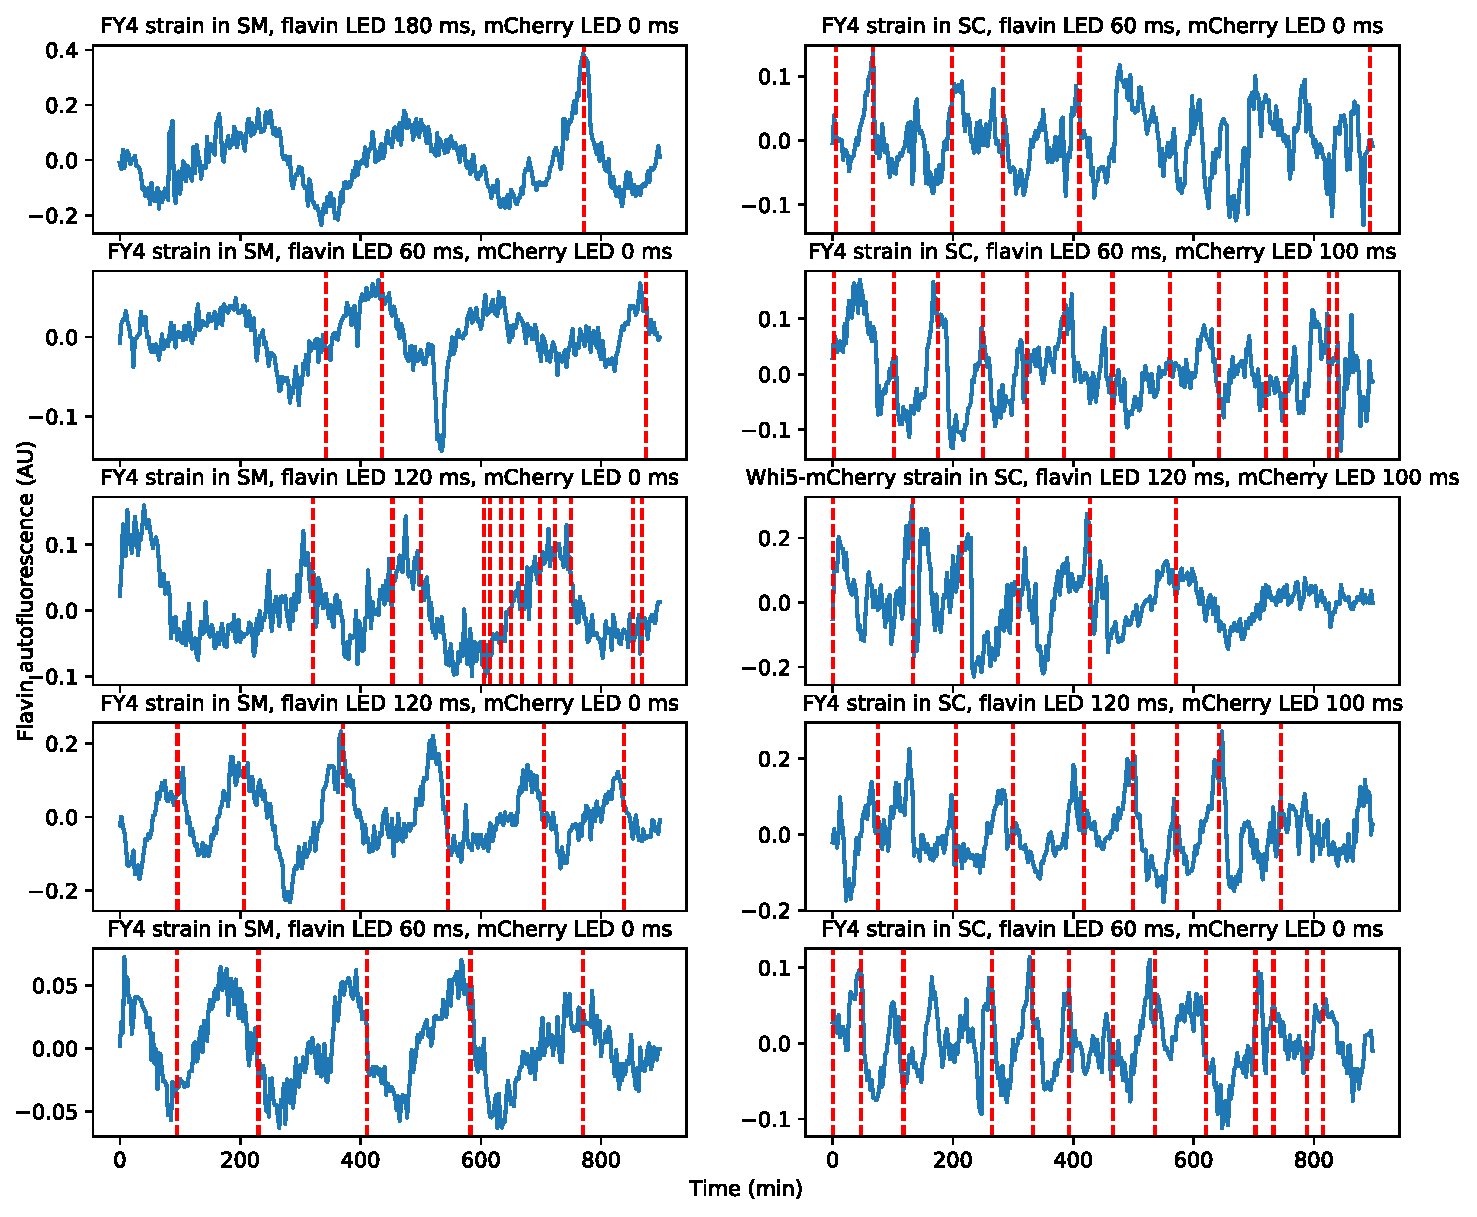
\includegraphics[width=\textwidth]{10m_ClassifierBestWorstTS}
  \caption{Classifier ranks time series by quality of oscillation.
    Left column shows `best' five and right column shows `worst' five.
    Blue: flavin autofluorescence, red: automatically identified birth}
  \label{fig:ClassifierBestWorstTS}
\end{figure}

\begin{figure}[htbp]
  \centering
  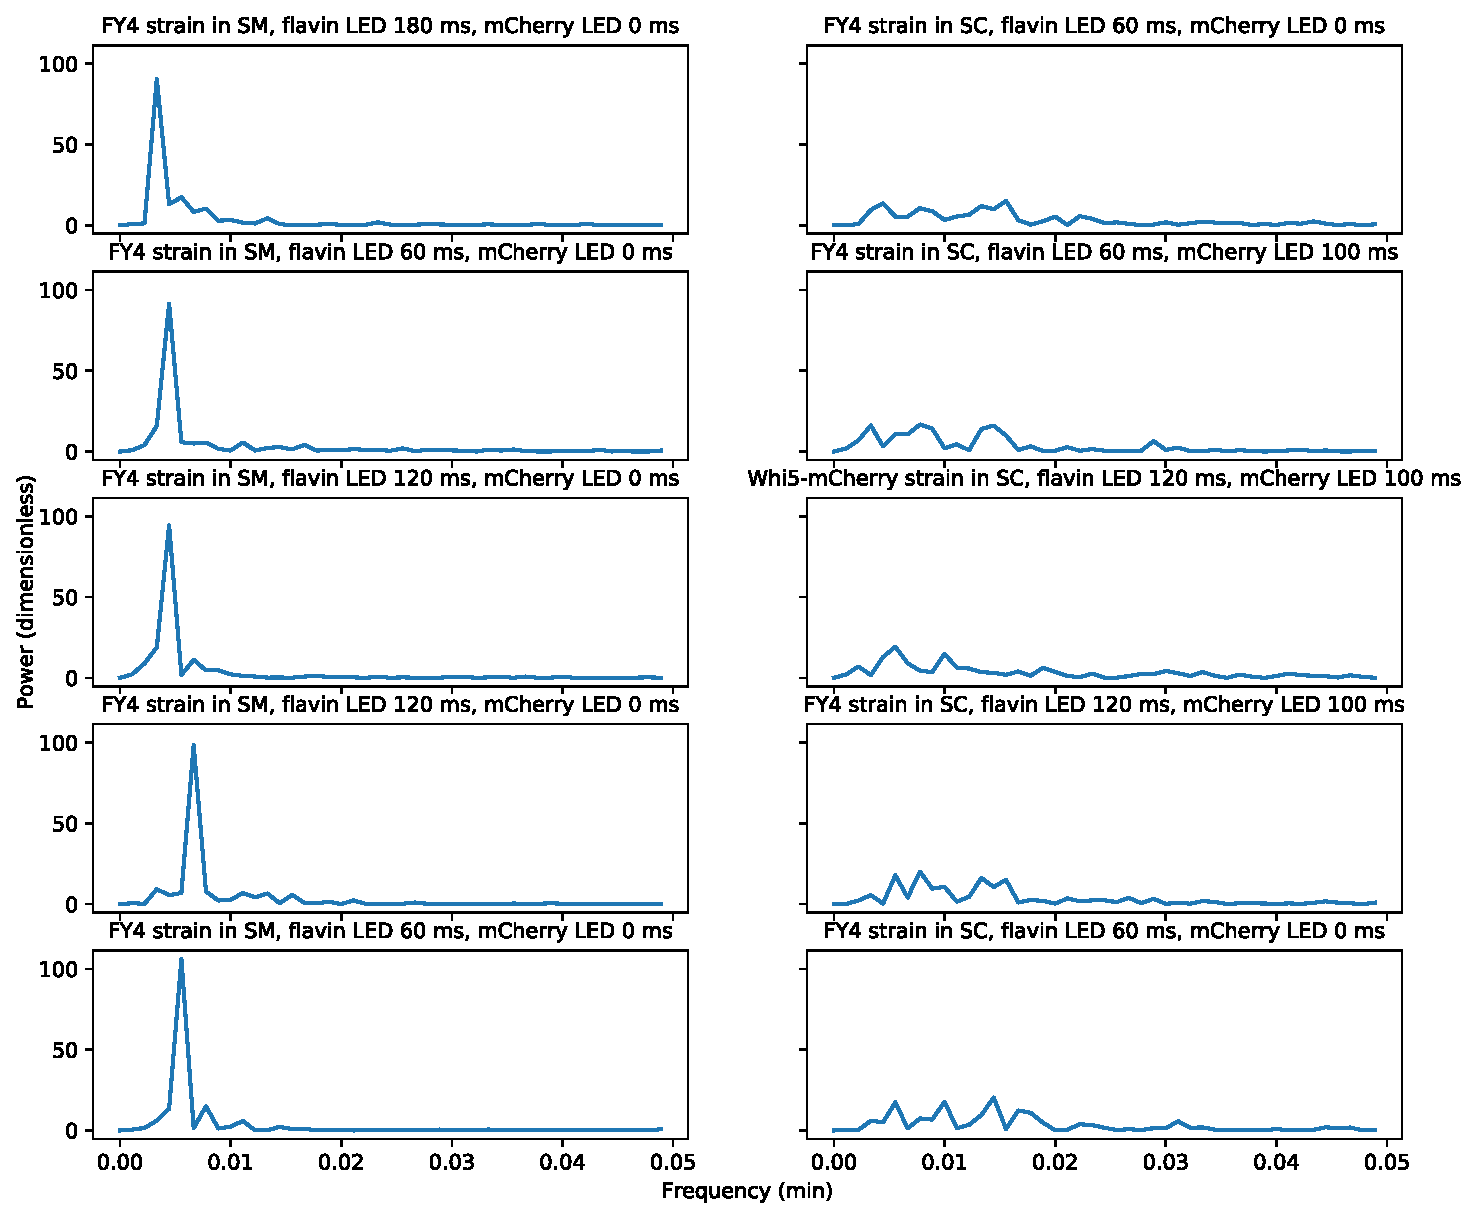
\includegraphics[width=\textwidth]{10m_ClassifierBestWorstPS}
  \caption{Highest peak of normalised classical periodograms is an inadequate proxy for quality of oscillations.
    Lines: normalised classical periodograms of time series in figure \ref{fig:ClassifierBestWorstTS}.}
  \label{fig:ClassifierBestWorstPS}
\end{figure}

Currently, the oscillation classifier has limited use.
It is difficult to characterise the time series of flavin autofluorescence using standard methods based on the data available.
The peak of the normalised classical periodogram inadequately captures the quality of the oscillations.

The oscillation classifier has one tuning parameter, the false discovery rate, and its value affects the proportion of time series classed as oscillating.

A reliable ground truth is needed to optimise the value of the false discovery rate so that the classification accuracy is maximised.
Because none of the experiments performed were ones from which oscillations were not expected, I lacked a reliable ground truth for the presence of oscillations.
I resorted to subjective judgements of whether a time series exhibited oscillations, and thus any optimised false discovery rate would have low reliability.

\subsection{Rhythmicity detection using model fitting}
\label{subsec:analysis-classification-ar}

The autoregressive model has been used before to characterise biological time series \parencite{zielinskiStrengthsLimitationsPeriod2014}.
This model is based on the assumption that each data point in the time series can be expressed as a linear combination of $N$ data points that precede it -- $N$ thus representing the order of the model.
This autoregressive model thus `smooths' the time series.
\parencite{jiaFrequencyDomainAnalysis2021} describe an application of the autoregressive model, based on the fact that there is an analytical solution for the periodogram based on this model.
In this publication, they use this paradigm to classify synthetic oscillations produced from a stochastic model of gene expression [CHECK IF ACCURATE.  AND LIFTING THE FIGURE FROM THEIR PAPER THAT SHOWS THIS WILL BE HELPFUL].
Specifically, the presence of a peak in the periodogram suggests that the time series is oscillatory.
And because the periodogram is produced from a analytical solution, you can compute the period and quantitfy the quality of the oscillation from this periodogram more easily than from a Fourier spectrum created from noisy data.

[FIGURE: EXAMPLE -- TIME SERIES ON THE LEFT, WITH SMOOTHED TIME SERIES, AND AR PERIODOGRAM ON THE RIGHT.]

In my investigations, very few time series within a dataset were classified as oscillatory using this method.
The problem is that there are no parameters that I can adjust to change the `tolerance' for detecting rhythmicity.
However, among the time series that it deems oscillatory, it guesses the frequency fairly well.

(Need: figures to summarise my investigation on population.  Probably need to re-do this on some datasets because it is poorly documented in my notes.)

Alternatively, I can treat the order of the model as a parameter, and perform model selection on it.

% This subsection needs better re-organisation.
% I've done some attempts by putting some headers in comments.
% But perhaps a better way is to draft some `summary' figures to show key takeaways, and then let the text flow accordingly.
\subsection{Machine learning approaches to classification}
\label{subsec:analysis-classification-ml}
% - Write results from classifier project (SVM, RF, etc.)

% Copied from org note: 'Using SVM with a population of cells', which isn't particularly well-written.
% ----------------------

% [TODO] Worth re-doing the whole experiment using better data, e.g. the data I'm actually using in the biological results chapter.

% DESCRIPTION OF DATA

For this section, I used data from BY4741 cells under 10 g/L glucose, before any nutrient changes.
% Probably no need to go into so much detail.
I removed the first 25 time points that is most likely cells adapting to microfluidic conditions.
I also removed time points after time point 168, when nutrient switching occurred.
I removed all time series with NaNs.
In total, there are 294 cells, each with 118 time points, spaced 5 minutes apart.

% DATA PROCESSING

% [TODO] Repeat experiment with Butterworth filter, rather than sliding window detrending

Figure ... shows a clear downwards trend (which I can't explain biologically yet). If an SVM model is trained using time points as features, there is a risk that the model recognises this trend rather than the presence of oscillations.
This plot highlights the risk: for some reason non-oscillating time series (hand-scored) tends to have a smaller gradient.
I thus detrended the data by generating a moving average with a sliding window size of 45 time points, and then dividing each data point by the moving average. I chose 45 time points because that covers ~3 cell division cycles.
However, there are caveats.
If the cell division cycle length differs, this window length should change; a spectral method (FFT, autoregressive) could give me an idea of what this cell division cycle length is.
Additionally, this decreases the number of time points --- there are now 98.

As the dynamic range of each time series are different from each other, I scaled each time series.
I used the standard scaler (\texttt{sklearn.preprocessing.StandardScaler()}), which makes each time series has mean 0 and standard deviation 1.

% LABELLING

Based on the processed (range restricted, detrending, normalised) data, I manually scored the 294 time series as non-oscillatory (label '0') or oscillatory (label '1').
Here, there are 211 oscillatory time series (72\%) and 83 non-oscillatory time series (28\%).
Thus, there is a slight class imbalance.

% SPLITTING

I chose 150 time series at random to be used as training data -- the rest becomes testing data.

% MODELS

I explored several model architectures: a support vector machine (SVM) and a random forest (RF) architecture.

I used an support vector classifier (SVC) with a radial bias kernel, using hyperparameters $C = 1$ and $\gamma = 1/(\mathrm{number of time points})$, and normalise features using the standard scaler.
For featurisation, I explored using time points as features, the time series' Fourier spectrum as features, and using \texttt{catch22} features.
I then evaluated the model using stratified five-fold cross-validation, using precision and recall as evaluation metrics.

Using time points as features, the metrics show that precision and recall is better than random, and stratified
five-fold cross-validation does not suggest overfitting (figure ...).

% Replace this with a bar plot.
% It's probably a good idea to combine all bar plots in this bit of the chapter into one figure with subfigures, so that it is easy to compare featurisation strategies.
\texttt{
     Precision 0.8127 Recall 0.7458\\
     Precision 0.8127 Recall 0.7458\\
     Precision 0.8036 Recall 0.7288\\
     Precision 0.8410 Recall 0.7966\\
     Precision 0.8966 Recall 0.8793\\
}

% Replace this with a bar plot
\texttt{
     Precision 0.5562 Recall 0.7458\\
     Precision 0.5562 Recall 0.7458\\
     Precision 0.5312 Recall 0.7288\\
     Precision 0.5312 Recall 0.7288\\
     Precision 0.5496 Recall 0.7414\\
}

Using the Fourier spectrum as features, precision and recall are comparative as with using time points as
features.
However, there seems to be greater variation in these measures.

% Replace this with a bar plot
\texttt{
     Precision 0.8700 Recall 0.8644\\
     Precision 0.9005 Recall 0.8983\\
     Precision 0.7676 Recall 0.7797\\
     Precision 0.8857 Recall 0.8644\\
     Precision 0.9517 Recall 0.9483\\
}

The spectra suggest that oscillatory cells exhibit a peak that is absent in non-oscillatory cells.
The peak corresponds to a period of 70~80 minutes.
This peak may explain the good precision \& recall scores.

For my last strategy of featurisation,
I employed the \emph{hctsa} toolbox \citep{fulcherHctsaComputationalFramework2017} to compute vectors of features for each time series.
This toolbox contains 7701 features defined from across the time series analysis literature.
I focused on the 22-feature \emph{catch22} subset of the original 7701 features (table \ref{tab:catch22}).
\citet{lubbaCatch22CAnonicalTimeseries2019} selected these 22 features because they minimise redundancy while maintaining classification performance across 93 test datasets.
This feature set excludes features that are dependent on mean or spread.

\begin{table}[htbp]
  \small
  \centering
  \begin{tabularx}{\linewidth}{bbS}
    \toprule
    Feature name & Description \\
    \midrule
    \texttt{DN\_\-HistogramMode\_\-5} & Mode of z-scored distribution (5-bin histogram) \\
    \texttt{DN\_\-HistogramMode\_\-10} & Mode of z-scored distribution (10-bin histogram) \\
    \texttt{SB\_\-BinaryStats\_\-mean\_\-longstretch1} & Longest period of consecutive values above the mean  \\
    \texttt{DN\_\-OutlierInclude\_\-p\_\-001\_\-mdrmd} & Time intervals between successive extreme events above the mean \\
    \texttt{DN\_\-OutlierInclude\_\-n\_\-001\_\-mdrmd} & Time intervals between successive extreme events below the mean \\
    \texttt{first\_\-1e\_\-ac} & First 1/e crossing of autocorrelation function \\
    \texttt{firstMin\_\-acf} & First minimum of autocorrelation function \\
    \texttt{SP\_\-Summaries\_\-welch\_\-rect\_\-area\_\-5\_\-1} & Total power in lowest fifth of frequencies in the Fourier power spectrum \\
    \texttt{SP\_\-Summaries\_\-welch\_\-rect\_\-centroid} & Centroid of the Fourier power spectrum \\
    \texttt{FC\_\-LocalSimple\_\-mean3\_\-stderr} & Mean error from a rolling 3-sample mean forecasting \\
    \texttt{CO\_\-trev\_\-1\_\-num} & Time-reversibility statistic, $\langle(x_{t+1} - x_t)^3\rangle_t$ \\
    \texttt{CO\_\-HistogramAMI\_\-even\_\-2\_\-5} & Automutual information, $m = 2, \tau = 5$ \\
    \texttt{IN\_\-AutoMutualInfoStats\_\-40\_\-gaussian\_\-fmmi} & First minimum of the automutual information function \\
    \texttt{MD\_\-hrv\_\-classic\_\-pnn40} & Proportion of successive differences exceeding $0.04\sigma$ \\
    \texttt{SB\_\-BinaryStats\_\-diff\_\-longstretch0} & Longest period of successive incremental decreases \\
    \texttt{SB\_\-MotifThree\_\-quantile\_\-hh} & Shannon entropy of two successive letters in equiprobable 3-letter symbolization \\
    \texttt{FC\_\-LocalSimple\_\-mean1\_\-tauresrat} & Change in correlation length after iterative differencing \\
    \texttt{CO\_\-Embed2\_\-Dist\_\-tau\_\-d\_\-expfit\_\-meandiff} & Exponential fit to successive distances in 2-d embedding space \\
    \texttt{SC\_\-FluctAnal\_\-2\_\-dfa\_\-50\_\-1\_\-2\_\-logi\_\-prop\_\-r1} & Proportion of slower timescale fluctuations that scale with DFA (50\% sampling) \\
    \texttt{SC\_\-FluctAnal\_\-2\_\-rsrangefit\_\-50\_\-1\_\-logi\_\-prop\_\-r1} & Proportion of slower timescale fluctuations that scale with linearly rescaled range fits \\
    \texttt{SB\_\-TransitionMatrix\_\-3ac\_\-sumdiagcov} & Trace of covariance of transition matrix between symbols in 3-letter alphabet \\
    \texttt{PD\_\-PeriodicityWang\_\-th0\_\-01} & Periodicity measure of \citet{wangStructureBasedStatisticalFeatures2007}   \\
    \bottomrule \\
  \end{tabularx}
  \caption{\emph{catch22} features, adapted from \citet{lubbaCatch22CAnonicalTimeseries2019}.
  }
  \label{tab:catch22}
\end{table}

Precision and recall are best with this set of features.

% Replace this with a bar plot
\texttt{
     Precision 0.8550 Recall 0.8475\\
     Precision 0.8628 Recall 0.8644\\
     Precision 0.8983 Recall 0.8814\\
     Precision 0.9525 Recall 0.9492\\
     Precision 0.9832 Recall 0.9828\\
}

Feature vectors seem to suggest that feature 10 (9 on the plots as arrays start from zero, \texttt{FC\_LocalSimple\_mean3\_stderr}, mean error from a rolling 3-sample mean forecasting) plays an important role in distinguishing the oscillatory and non-oscillatory time series.
[EXPLAIN WTF IS FC\_Local...]

[SOME FIGURES MAY BE USEFUL HERE.]

% ADAPTATION OF SVM: PREDICT PROBABILITIES
I extended the support vector classifier by using the \texttt{predict\_proba = True} option [PLEASE REPLACE THIS WITH AN ACTUAL, VERBOSE EXPLANATION] so that the model computes the probability that a time series is oscillatory, rather than assign one of two outputs.

The distribution of probabilities falls in a U-shape, which is good.

[FIGURE: U-SHAPE HISTOGRAM FROM AC2022 POSTER.  ALSO INCLUDE THE RESULT FROM RANDOMLY ASSIGNING LABELS, WHICH SHOULD NOT GIVE A U-SHAPE, AS A CONTROL TO SHOW THAT THE MODEL IS ACTUALLY GOOD].

In addition, these probabilities can also serve as a score for the quality of oscillations, as illustrated by examples.

[FIGURE: GALLERY OF TIME SERIES WITH 0\%, 20\% ... 100\% PROBABILITY OF OSCILLATION]

% I mention modularity clustering before its appropriate section here.
% I can create a reference to that section, or move this paragraph to that section and re-word it a bit so it fits the logical flow.
The \texttt{catch22} features seem to function best so far.
It makes sense -- given that I could plot cells in \texttt{catch22} feature space and perform modularity clustering, an SVM model based on drawing a `lane' between two clouds of points in \texttt{catch22} feature space should work.
Furthermore, the publication that describes \texttt{catch22} features \parencite{lubbaCatch22CAnonicalTimeseries2019} has tested the features' ability to categorise time series across multiple large datasets.

(Better discussion here.  Sum up key points and discuss caveats.  Will probably be easier once I restructure this subsection.)

\section{Characterisation: I have one time series -- what properties does it have?}
\label{sec:analysis-characterisation}

The importance of characterising my time series is that I can quantify how my yeast metabolic cycles respond to genetic and nutrient perturbations.
Here, I discuss characterising periods, phases, and amplitudes of the oscillations.
Note that I discuss many of the same non-machine learning methods as I did for the classification section -- such methods are often developed for characterisation but offer features that are useful for classification, but it makes more sense in my thesis to order it this way because you'd usually try to filter out the non-oscillatory time series before trying to grab properties of the oscillatory ones.
Then I will discuss the merit of combining several methods, given the limitations of analysing noisy biological time series that I have found.
Characterisation is also intimately related to classification, in particular the machine learning methods: these methods can be adapted to tell apart different strains (presumably of different shapes) rather than telling apart oscillatory and non-oscillatory time series.

% Literature review subsection
% STEAL IDEAS FROM: ZIELINSKI ET AL. 2014
\subsection{Periods, phases, amplitudes}
\label{subsec:analysis-characterisation-quantities}

% Copied from meeting with Zielinski.
% TODO with this:
% - adapt to prose
% - support with evidence, e.g. discussion points from his paper and others
Period
\begin{itemize}
\item Easy to obtain a fixed number from data because it is well-defined.
\end{itemize}

Shape
\begin{itemize}
\item Difficult to analyse and assign a meaningful quantitative measure.  Much easier to describe by eye.
\begin{itemize}
\item Often expressed as \emph{skewness} -- after treating one oscillation/peak as a distribution.  Such a peak can be obtained by averaging individual oscillations in a population.
\end{itemize}
\item My oscillations all have similar shapes: triangular \& symmetrical.
\end{itemize}


Phase
\begin{itemize}
\item Tricky to obtain a fixed number from data.  The phase angle obtained can often be noisy/varied.
\begin{itemize}
\item Period estimator will always give an error.
\item Modular arithmetic needed.
\item We need multiple replicates -- plot populations of time series and see if they overlap.
\end{itemize}
\item Need an original/reference phase, which I \emph{need to choose} and it is not always super clear.  There is usually damping compared to this.
\item Phase depends on the period too.  It could be:
\begin{itemize}
\item Absolute (hours), or
\item With respect to the period (radians).  Normally, use this one, unless I am interested in response to a treatment.
\end{itemize}
\end{itemize}

Amplitude
\begin{itemize}
\item Easier to do and easy to explain.
\item Likely the least important characteristic.
\item Fit a cosine.  Works if shape doesn't change a lot.  Bad if oscillations are skewed.
\end{itemize}

Of these, finding the period is the easiest to do and most pertinent for my investigation of the yeast metabolic cycle, so I'm going to focus on this.
Here is a review of some methods used in \textcite{zielinskiStrengthsLimitationsPeriod2014}

% Copied from meeting with Zielinski.
% I probably need to try out at least the first two
FFT NLLS
\begin{itemize}
\item Try this first.  Common with circadian people.
\item Enforces shapes.  Chooses number of sinusoids that fit the shape best, up to 5.  Then reports the best component.
\item Has confidence intervals, e.g. relative amplitude error ($\leq$ 50\% is good).
\item Skewness doesn't affect period.
\end{itemize}

MFourFit
\begin{itemize}
\item Uses harmonics.  Can use the harmonics to describe shapes of oscillations.
\item Fits only 1 component, unlike FFT NLLS.  Period and phase interpreted from the main sinusoid component.
\item Enforces shapes.
\item Skewness doesn't affect period.
\end{itemize}

MESA
\begin{itemize}
\item Fit autoregressive model then gets period from it.
\item Scours periods, then selects model that does best.
\item Empirically does well and fast.
\item Is based on a very different principle than MFourFit, so if both methods agree on the value of the period, then we can be confident that we have the correct period.
\end{itemize}

Lomb-Scargle periodogram
\begin{itemize}
\item Fits one sinusoid, assumes a period.
\item Choose one that gives least error.
\end{itemize}

As I've already discussed the FFT and autoregressive model, I am now going to focus on the autocorrelation function.

\subsection{Autocorrelation function}
\label{subsec:analysis-characterisation-acf}

This report explores the cross-correlation and autocorrelation functions, adapted to a population of noisy time series, as a method to characterise the periodicity and heterogeneity of oscillatory time series.  The report does so through simulated oscillatory time series based on models with very well-characterised behaviours: a harmonic oscillator and a relaxation oscillator.  The hope is that these synthetic time series can adequately model flavin fluorescence oscillations and the behaviour of histones during the cell division cycle.

\subsubsection{Mathematical basis}
\label{subsubsec:analysis-correlation-maths}
% \subsubsection{Simulating oscillators}
% \label{sec:analysis-correlation-maths-osc}

I choose the harmonic oscillator and the FitzHugh-Nagumo model to investigate because they are simple, well-characterised, and mimic the biological time series that I am interested in.  Here I detail the rationale behind my choices and describe the oscillators I choose.

\begin{enumerate}
\item Harmonic oscillator
\label{sec:org7f23d98}

I choose the harmonic oscillator because it is the simplest case of an oscillator, with only one parameter.  Namely:

\(\frac{d^{2}y}{dt^{2}} = -\omega^{2}y\)

where \(y\) represents displacement and \(\omega\) represents the angular frequency.

Or written in the form of a system of first-order differential equations:

\(\frac{dy}{dt} = v\)

\(\frac{dv}{dt} = -\omega^{2}y\)

This model produces time series \(y(t)\) that is a sinusoid, i.e.

\(y(t) = A sin(\omega{}t + \phi)\)

where \(A\) and \(\phi\) are determined by initial conditions.

\item FitzHugh-Nagumo model
\label{sec:orgdffb616}

I choose the FitzHugh-Nagumo model because it is a well-characterised relaxation oscillator that can model a more complicated time series, while still being simple, with only four parameters.

The FitzHugh-Nagumo model was developed to model an excitable system, such as a neuron.  The model is described as a system of first-order differential equations (citation needed):

\(\frac{dv}{dt} = v - \frac{v^3}{3} - w + RI_{\mathrm{ext}}\)

\(\tau \frac{dw}{dt} = v + a - bw\)

where the variables include:
\begin{description}
\item[{\(v\)}] membrane voltage
\item[{\(w\)}] linear recovery variable
\end{description}

and the parameters include \(RI_{\mathrm{ext}}\) (external stimulus), \(\tau\), \(a\), and \(b\) [describe what they are and how they control the model].

This model produces time series \(v(t)\) that is a relaxation oscillator [why relaxation oscillator?].
\end{enumerate}

% \subsubsection{Generating noise}
% \label{sec:analysis-correlation-maths-noise}

Biological time series, and certainly the ones that I study, have noise.  So, it makes sense to add noise to our models as well, because noise affects the behaviour of models and the analysis methods applied to the time series generated by our models.

Here, I describe two types of noise I investigate and how to integrate them with my models.

\begin{enumerate}
\item Gaussian noise
\label{sec:org38e563f}

[To clarify: should I use white noise or Gaussian noise?  These are not equivalent, but can overlap.  Current code generates Gaussian noise.]

I use (white) Gaussian noise as it is the simplest, first-approach case.  This noise is generated by randomly drawing samples from the normal distribution \(\mathcal{N}(1,0)\).

[Figure may be useful, but only to contrast with Gillespie noise.]

\item Gillespie noise from birth-death process
\label{sec:orge5d486b}

I use Gillespie noise because it's the same type of noise from biological systems [citation needed, maybe Wilkinson `Stochastic Modelling for Systems Biology'].

The Gillespie noise was generated as follows, using example parameter values:

Define the birth-death process: birth rate \(k_{0} = 5\) and death rate \(d_{0} = 0.05\).  Set a stochastic simulation with final time of 1500, and put the trajectories on a grid with regularly-spaced time points, 1000 time points in this case.

Each trajectory took some time to reach steady state (see image below), so the latter half was taken, assuming it is in steady-state:
\begin{center}
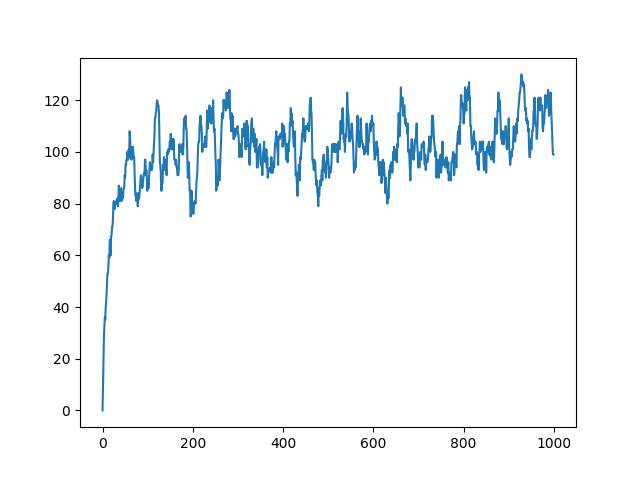
\includegraphics[width=.9\linewidth]{gillespie.png}
\end{center}

Here, the steady-state mean is equal to the steady-state variance, which is equal to \(k_{0}/d_{0}\).

I normalised this trajectory by subtracting the mean (\(k_{0}/d_{0}\)) and then dividing by \(\sqrt{1/d_{0}}\) to create Gillespie noise with mean 0 and standard deviation \(\sqrt{k_{0}}\) -- this is so that changes in \(k_{0}\) affect the noise amplitude.

As an example, I show 3 trajectories of Gillespie noise using the initial parameters I set:
\begin{center}
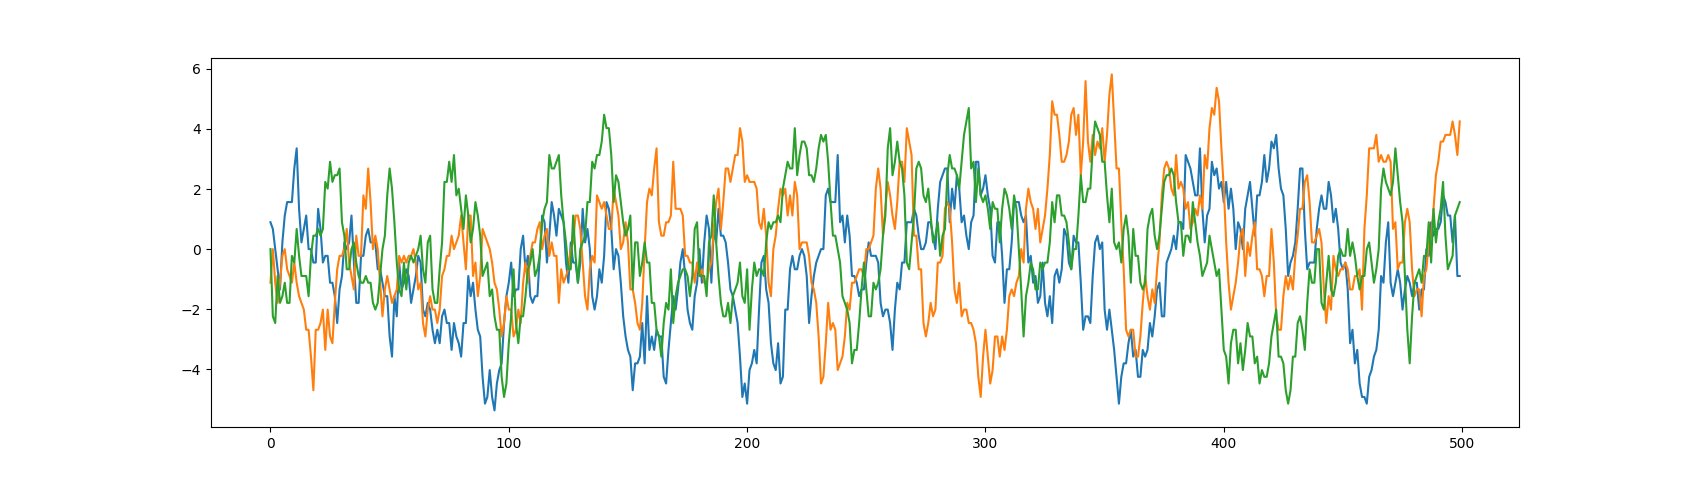
\includegraphics[width=.9\linewidth]{gillespie_noise_samples.png}
\end{center}

Alternatively, Gillespie noise can be parametrised in the form of standard deviation of noise amplitude \(A = \sqrt{k_{0}/d_{0}}\) and noise timescale \(\tau = 1/d_{0}\).

\item Adding noise
\label{sec:org03ea61a}

Approach: add to time series (simple sum).
\end{enumerate}

\subsubsection{Computing autocorrelation and cross-correlation}
\label{sec:analysis-correlation-maths-algorithm}

TODO: Describe the algorithm using mathematical notation (copy from BABY paper).  Mention that autocorrelation is a special case of cross-correlation.

TODO: Justify deviations from the `classical' mathematical definition, e.g. how a population of signals is treated, subtracting mean, etc. (This will be obvious when I write down the `classical' definition).  Also talk about: stationary option (mean across replicates and time points).

\subsection{Results}
\label{sec:analysis-correlation-results}

\begin{enumerate}
\item Autocorrelation on sinusoids
\label{sec:org2fe8e39}

\begin{enumerate}
\item Without noise: signals must be out of phase
\label{sec:orgeef3284}

Need to make sure that we understand the autocorrelation function, so we start from the simplest case: the sinusoid.  Want to understand what processes control the shape of autocorrelation and cross correlation functions.

In-phase sinusoids to be used as input data:
\begin{center}
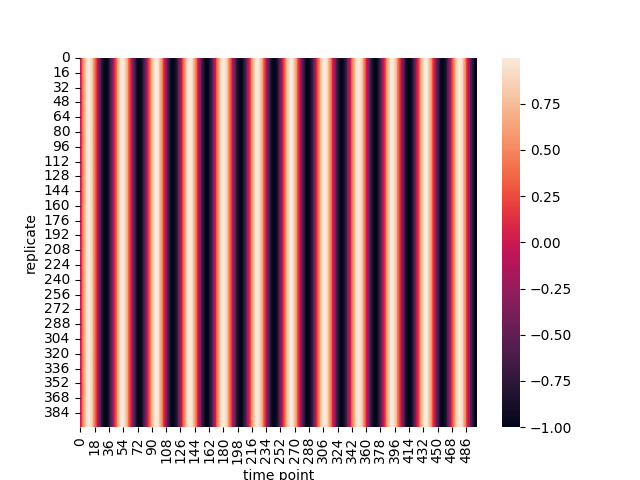
\includegraphics[width=.9\linewidth]{sinusoids_inphase.png}
\end{center}

Autocorrelation functions of in-phase sinusoids are identical and only show noise, therefore uninformative:
\begin{center}
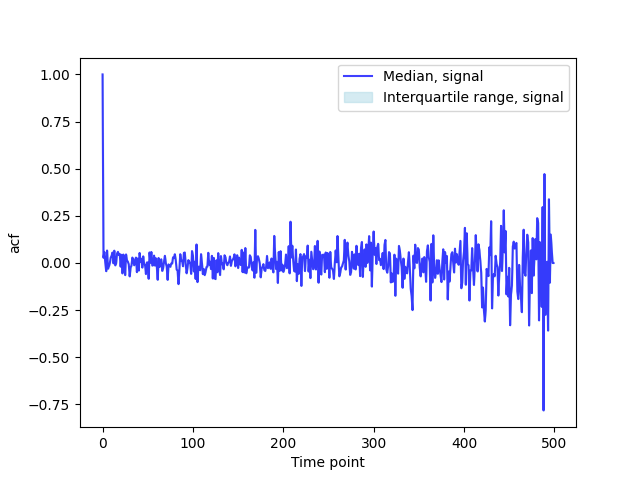
\includegraphics[width=.9\linewidth]{sinusoids_inphase_acf.png}
\end{center}

As the underlying dynamic process is stationary with a constant mean, we can modify our calculation of the autocorrelation function so that the mean is calculated over time and replicates.  This modification allows us to deal with in-phase sinusoids, with this results confirming this:
\begin{center}
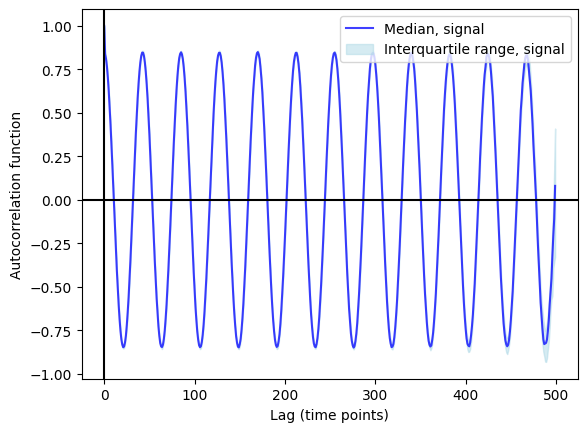
\includegraphics[width=.9\linewidth]{sinusoids_inphase_acf_stationary.png}
\end{center}

A different set of input data is then generated with a random initial phase sampled from the distribution \(Unif[0,2\pi)\).
\begin{center}
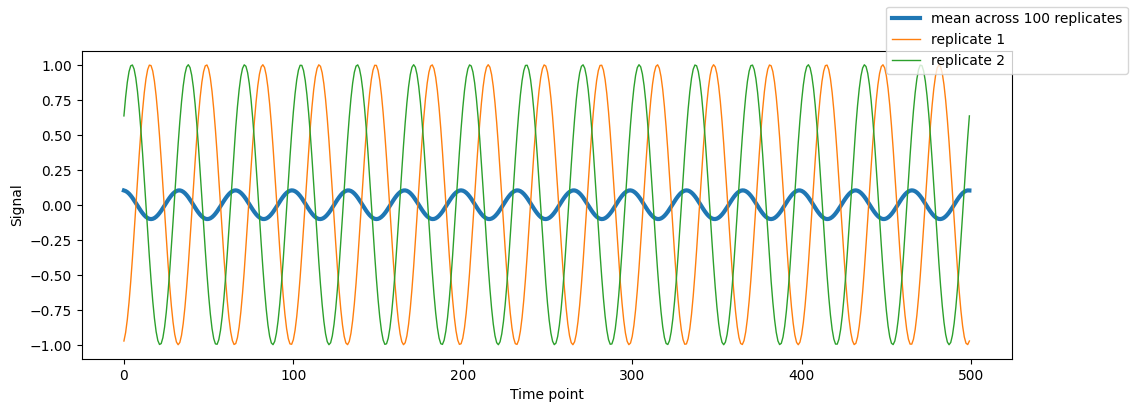
\includegraphics[width=.9\linewidth]{sinusoids_outofphase.png}
\end{center}

Autocorrelation functions of out-of-phase sinusoids resemble a cosine wave with an amplitude of 1, which is how they should be in theory.
As a check, each oscillation of the autocorrelation function corresponds to the period of the source oscillations:
\begin{center}
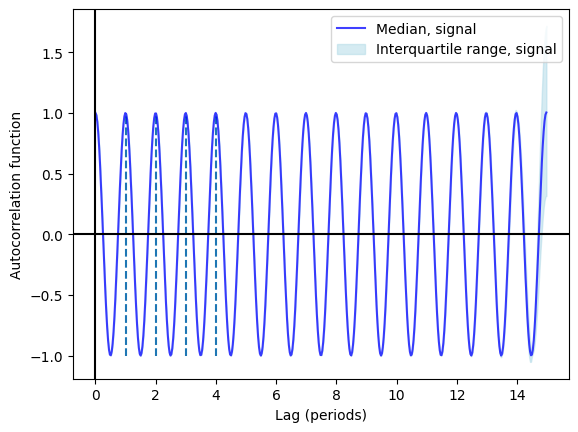
\includegraphics[width=.9\linewidth]{sinusoids_outofphase_acf_corrected.png}
\end{center}

\item Mixed frequencies
\label{sec:orgbc4bd46}

As additional investigation on a population with mixed frequencies: 200 sinusoids of frequency 0.03 and 20 sinusoids of frequency 0.04

Autocorrelation function, lag axis scaled by frequency 0.03:
\begin{center}
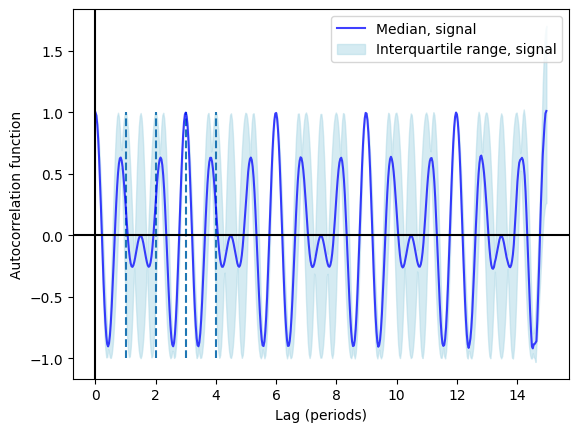
\includegraphics[width=.9\linewidth]{sinusoids_mixed_acf_freq0p03.png}
\end{center}

Autocorrelation function, lag axis scaled by frequency 0.04:
\begin{center}
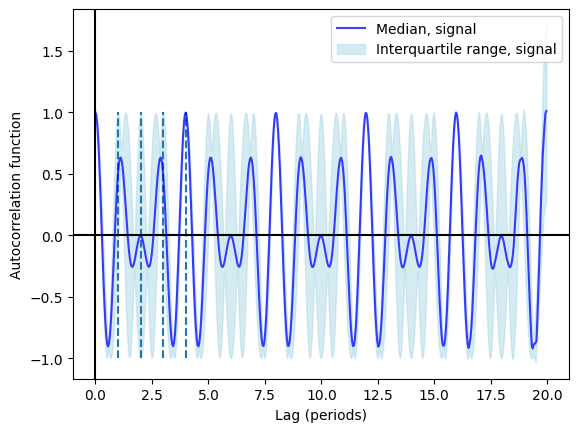
\includegraphics[width=.9\linewidth]{sinusoids_mixed_acf_freq0p04.png}
\end{center}

\item With Gaussian noise
\label{sec:org07e90f1}

In-phase sinusoids with Gaussian noise (standard deviation 0.3), to be used as input data:
\begin{center}
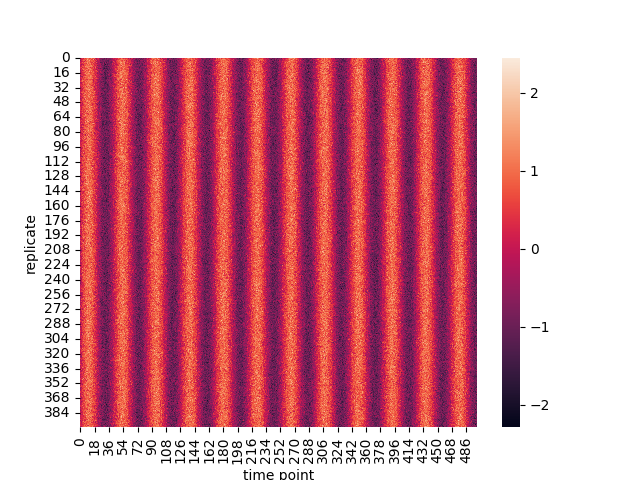
\includegraphics[width=.9\linewidth]{noisysinusoids_inphase.png}
\end{center}

The variation between autocorrelation functions of each in-phase sinusoids is only due to the Gaussian noise added, and therefore uninformative:
\begin{center}
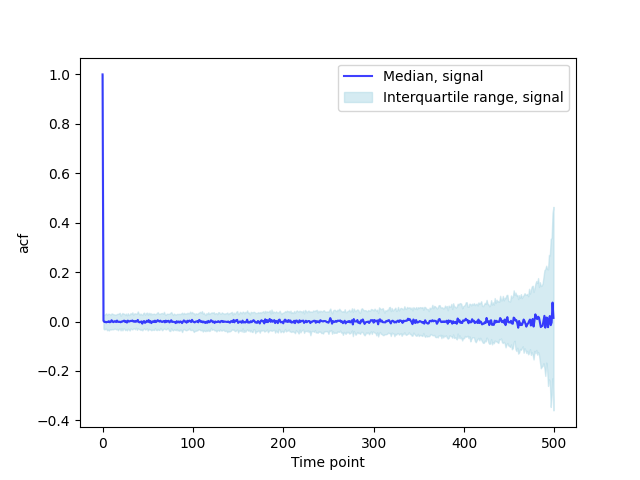
\includegraphics[width=.9\linewidth]{noisysinusoids_inphase_acf.png}
\end{center}

Again, we can used the modified calculation because the underlying dynamic process is stationary with a constant mean.  In this case, the results are similar to as before (without Gaussian noise).
\begin{center}
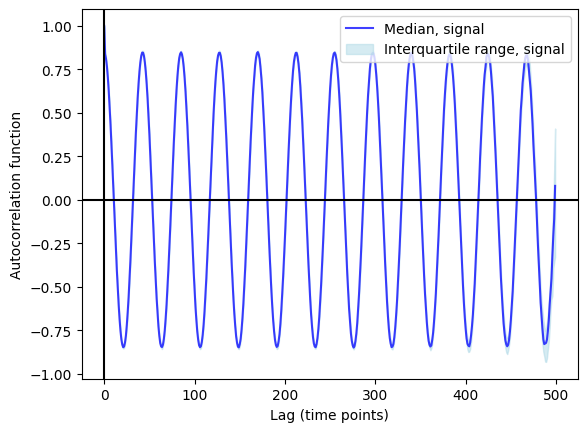
\includegraphics[width=.9\linewidth]{noisysinusoids_inphase_acf_stationary.png}
\end{center}

We repeat the investigation but with a random initial phase:
\begin{center}
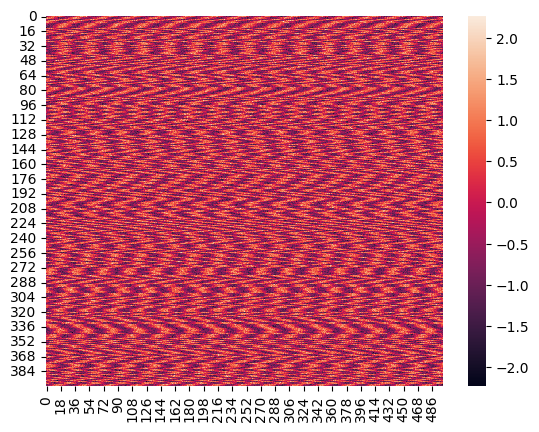
\includegraphics[width=.9\linewidth]{noisysinusoids_outofphase.png}
\end{center}

Autocorrelation functions of out-of-phase noisy sinusoids resemble a cosine wave with an amplitude of 1, which is how they should be in theory:
\begin{center}
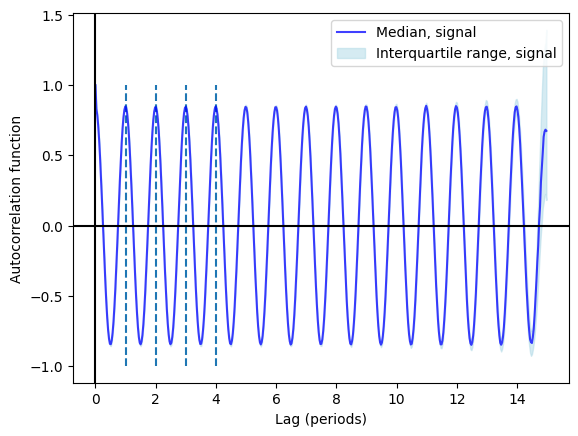
\includegraphics[width=.9\linewidth]{noisysinusoids_outofphase_acf.png}
\end{center}

To emphasise the effect of noise, here I repeat the analysis with noise standard deviation 3.0:
\begin{center}
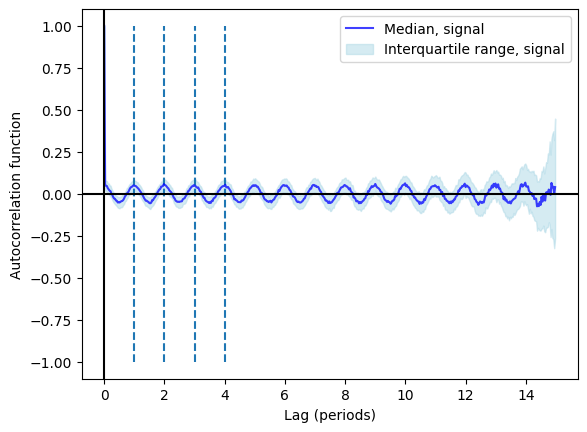
\includegraphics[width=.9\linewidth]{verynoisysinusoids_outofphase_acf.png}
\end{center}

Here, the amplitude of the autocorrelation functions are decreased and the variation between each time series' autocorrelation function is increased.  And at higher lag times, this variation is greater because there is less data that is used.  This is exemplified in this plot:
\begin{center}
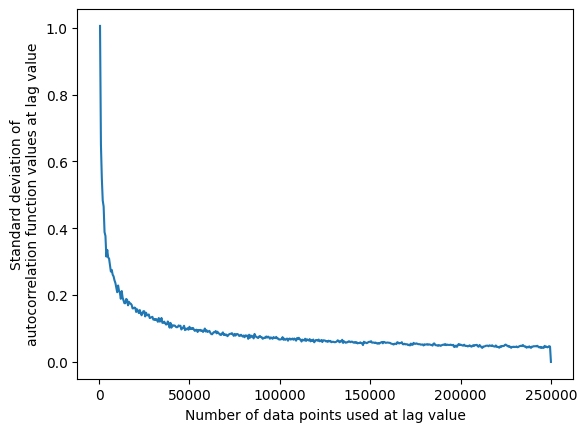
\includegraphics[width=.9\linewidth]{lag_datapoints_vs_stddevacf.png}
\end{center}

  \item With Gillespie noise
\label{sec:org30f0d40}

\begin{enumerate}
\item Approach
\label{sec:orgd554193}

Create an oscillator.  Simulate Gillespie noise using a birth-death process, then add to oscillator.

Vary timescale and amplitude of noise with respect to signal.

\item Constructing replicates
\label{sec:orge2355a3}

I performed 100 replicates of a sinusoid of frequency 0.03 with different phases.  I then generated 100 trajectories to Gillespie noise as described above, and added them together to produce the simulated replicates.  This gave the following mean across replicates and autocorrelation function:
\begin{center}
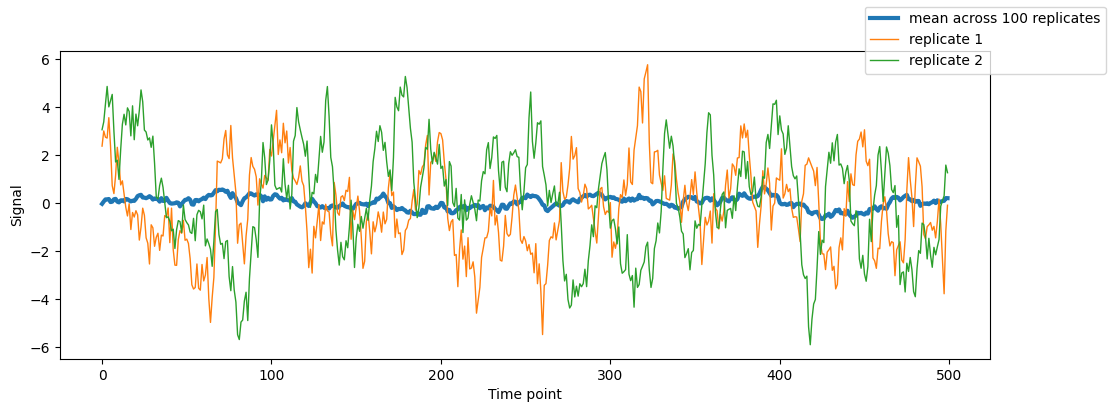
\includegraphics[width=.9\linewidth]{gillespie_k5_d0p05_mean.png}
\end{center}
\begin{center}
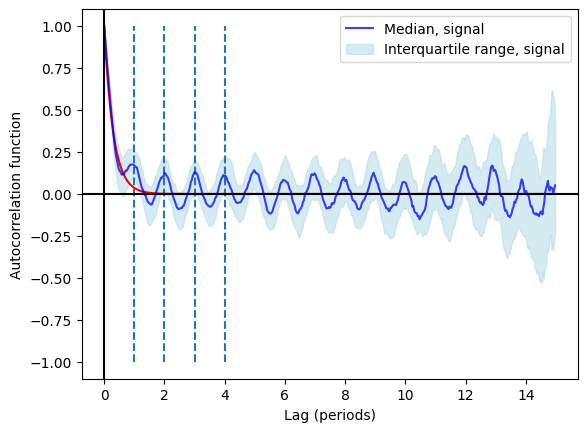
\includegraphics[width=.9\linewidth]{gillespie_k5_d0p05_acf.png}
\end{center}

As a check, I drew an exponential decay function (\(y = e^{-2d_{0}T}\), where \(T\) represents lag) to the autocorrelation function.  The exponential function should fit the median autocorrelation function.

In addition, the oscillations in the autocorrelation function should occur every period of the sinusoid, as already shown above.

\item Varying timescale of noise
\label{sec:org7d5f612}

Changing the death rate \(d_{0}\) to 0.5 -- higher death rate seems to decrease the decay timescale for the autocorrelation function:
\begin{center}
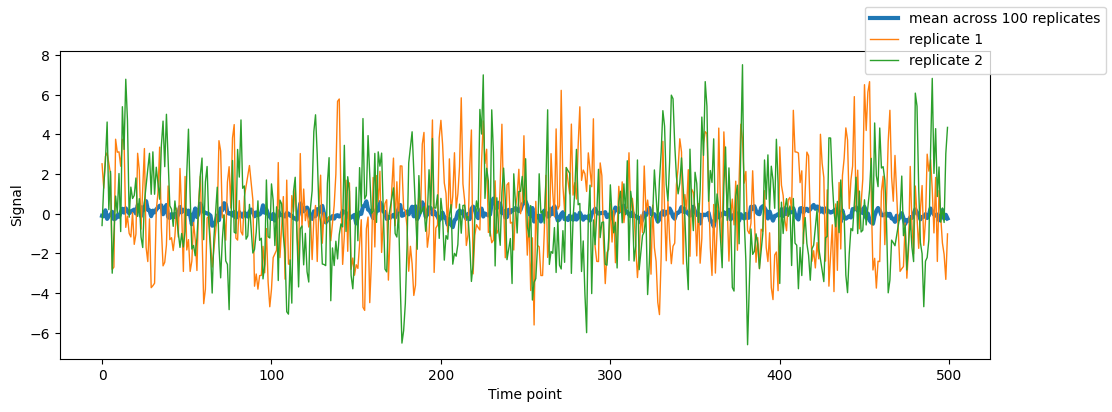
\includegraphics[width=.9\linewidth]{gillespie_k5_d0p5_mean.png}
\end{center}
\begin{center}
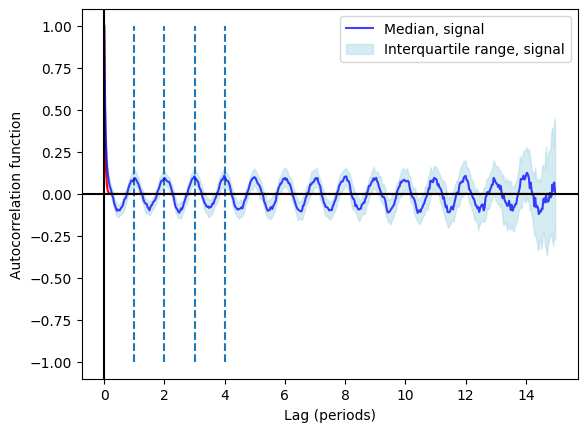
\includegraphics[width=.9\linewidth]{gillespie_k5_d0p5_acf.png}
\end{center}

Changing the death rate \(d_{0}\) to 0.005.  Lower death rate seems to introduce long-term trends in the simulated signals.  It also increase the decay timescale for the autocorrelation function and increases the variation between autocorrelation functions between replicates.
\begin{center}
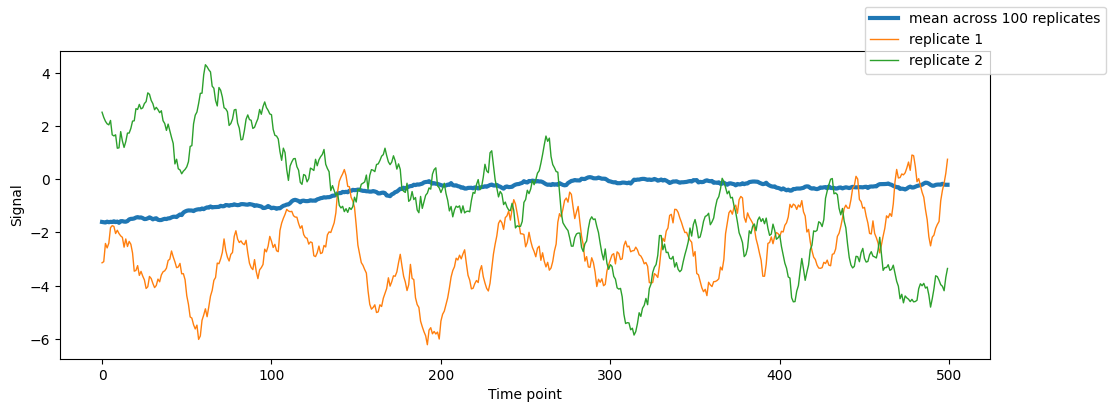
\includegraphics[width=.9\linewidth]{gillespie_k5_d0p005_mean.png}
\end{center}
\begin{center}
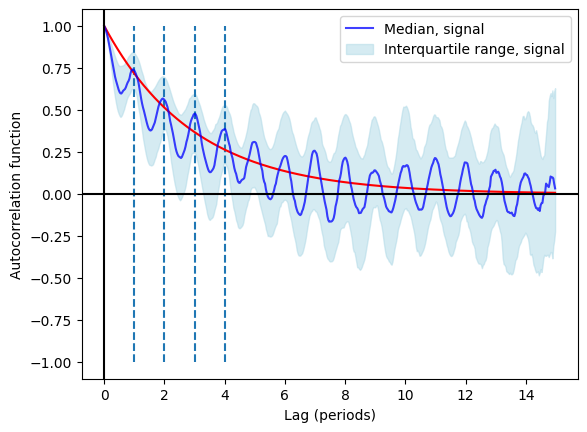
\includegraphics[width=.9\linewidth]{gillespie_k5_d0p005_acf.png}
\end{center}

I then fit exponential decay functions of the form \(y = (1-C)e^{-kT}+C\), using non-linear least squares, to the mean autocorrelation function, the peaks of this mean function, and the troughs of these functions.  As an example:
\begin{center}
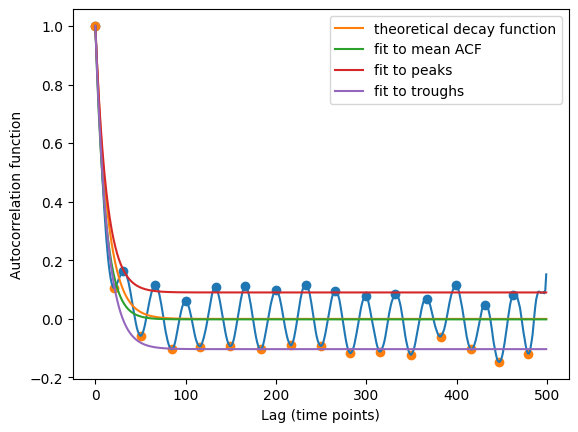
\includegraphics[width=.9\linewidth]{acf_fit_example.png}
\end{center}

In theory, the decay rate \(k\) should scale linearly with the death rate \(d_{0}\).  Sweeping across values of \(d_{0}\), I confirm that is the case.  This figure thus summarises the effect of death rate in decay timescale:
\begin{center}
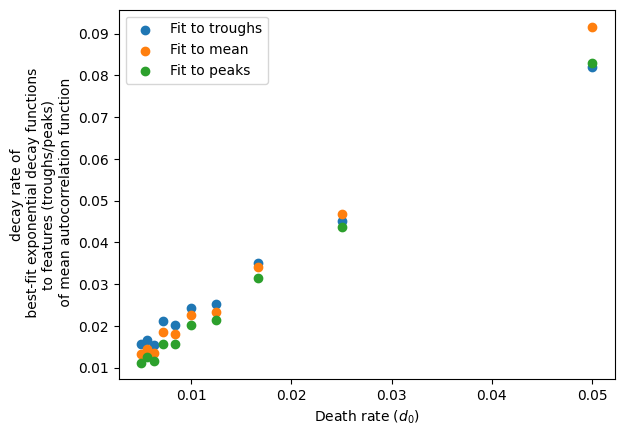
\includegraphics[width=.9\linewidth]{deathrate_vs_decay.png}
\end{center}

To quantify the variation between autocorrelation functions between replicates, I computed the standard deviation autocorrelation function values at each lag:
\begin{center}
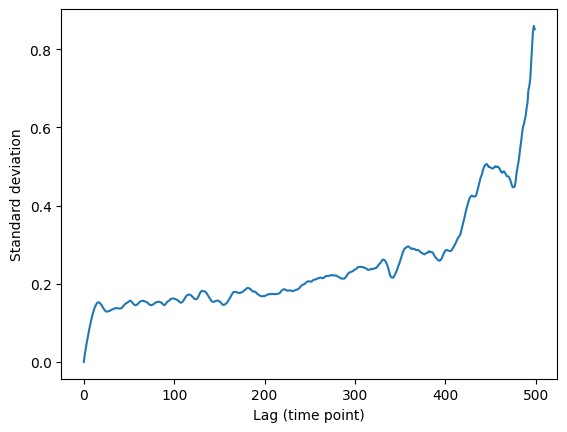
\includegraphics[width=.9\linewidth]{stddevauc_example.png}
\end{center}

and then computed the area under this curve as a proxy for the variation between replicates.

As the noise timescale \(1/d_{0}\) increased, this area under curve increased:
\begin{center}
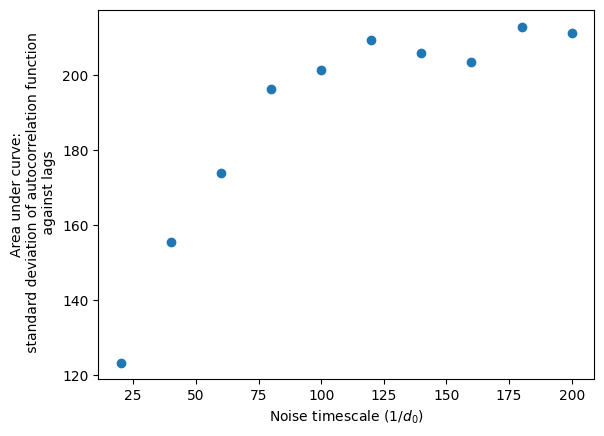
\includegraphics[width=.9\linewidth]{deathrate_vs_auc.png}
\end{center}

\item Varying amplitude of noise
\label{sec:org4110edb}

Changing the birth rate \(k_{0}\) to 1.  Lower birth rate decreases the amplitude of noise.  It also makes the autocorrelation function more robust and decreases the variation between replicates.
\begin{center}
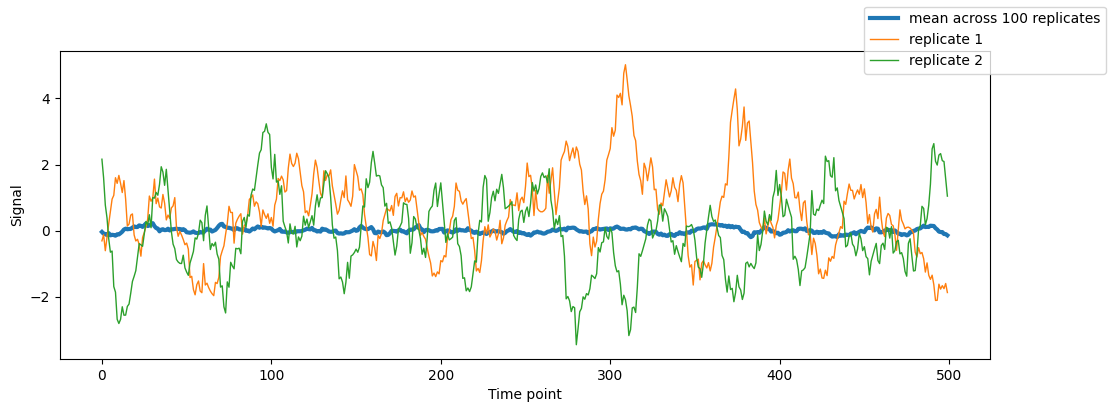
\includegraphics[width=.9\linewidth]{gillespie_k1_d0p05_mean.png}
\end{center}
\begin{center}
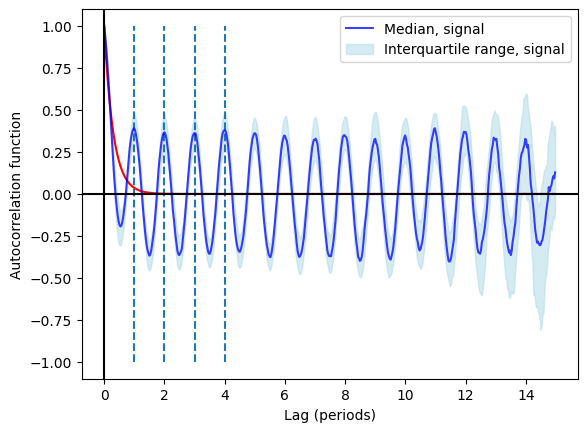
\includegraphics[width=.9\linewidth]{gillespie_k1_d0p05_acf.png}
\end{center}

Changing the birth rate \(k_{0}\) to 25.  Higher birth rate increases the amplitude of noise.   It also makes the autocorrelation function less robust and increases the variation between replicates.
\begin{center}
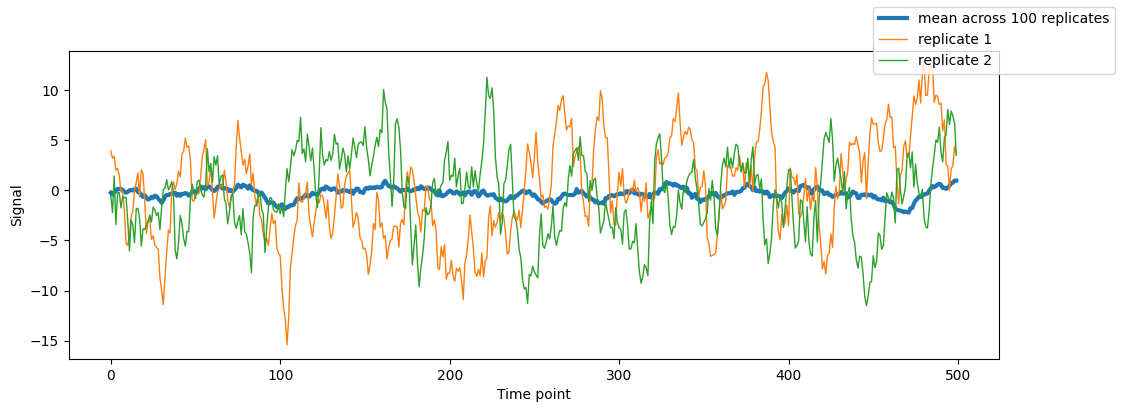
\includegraphics[width=.9\linewidth]{gillespie_k25_d0p05_mean.png}
\end{center}
\begin{center}
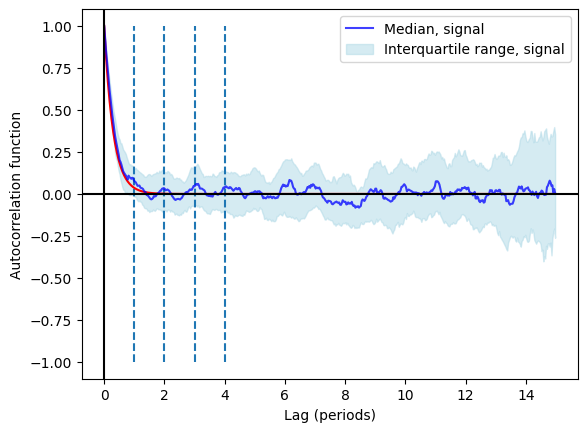
\includegraphics[width=.9\linewidth]{gillespie_k25_d0p05_acf.png}
\end{center}

Similar to previously, I fit \(y = (1-C)e^{-kT}+C\), using non-linear least squares, to the mean autocorrelation function, the peaks of this mean function, and the troughs of these functions.

To show that the amplitude of the oscillations in the autocorrelation function decreases as the birth rate increases, I plotted the fitted \(C\) (y-displacement) parameters against the noise amplitude \(k_{0}/d_{0}\):
\begin{center}
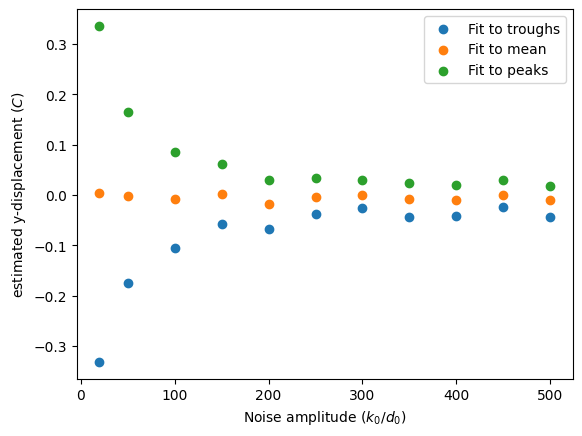
\includegraphics[width=.9\linewidth]{birthrate_vs_ydispl.png}
\end{center}

Additionally, I subtracted the decay equation fitted to the mean autocorrelation function from the mean autocorrelation function.  The residuals obtained represent the oscillations within the autocorrelation function:
\begin{center}
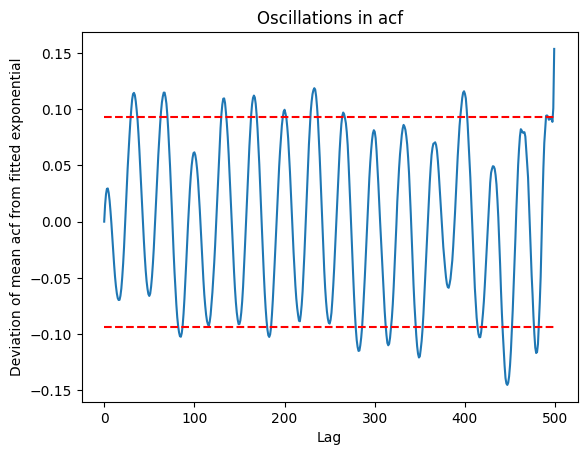
\includegraphics[width=.9\linewidth]{residual_example.png}
\end{center}

This can be subject to further analysis.  Here, I estimated the amplitude of these oscillations based on the height of the peak in its Fourier transform (\(A = \sqrt{2y}\)), shown as red dotted lines.

This amplitude can be computed as the amplitude of noise varies, and I show that as the noise amplitude increases, the amplitude of the oscillations in the autocorrelation function decreases:
\begin{center}
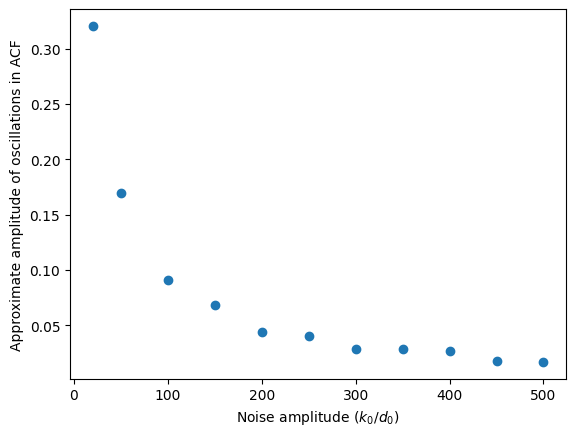
\includegraphics[width=.9\linewidth]{birthrate_vs_acfamp.png}
\end{center}

To quantify the variation between autocorrelation functions between replicates, I computed the standard deviation autocorrelation function values at each lag and the area under this curve, as previously.  My calculations demonstrate that higher birthrate increases the variation between replicates:
\begin{center}
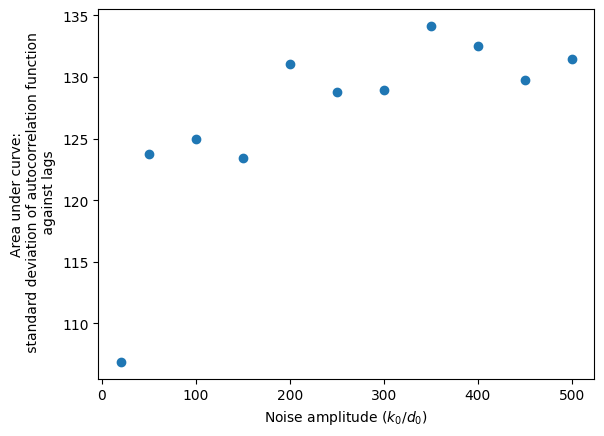
\includegraphics[width=.9\linewidth]{birthrate_vs_auc.png}
\end{center}

\item Conclusions
\label{sec:orge2a0d5d}

If a population of replicate oscillatory time series is modelled with the sum of sinusoids and Gillespie noise, then the birth rate and death rate can control the shape of the autocorrelation function.  The death rate controls the timescale of noise and thus how fast the autocorrelation decays as lag increases.  The birth rate controls the amplitude of noise and thus controls how robust the autocorrelation function is.  Knowing these relationships, one can deduce noise parameters from the autocorrelation functions of real signals.

Gillespie noise seems to model the noise I observe in experiments better than white noise, and I can even tune the parameters to create a better fit.
\end{enumerate}

\item Compare with biological oscillator
\label{sec:orgbccdb4a}

My intention is to have it model oscillations of flavin fluorescence that act as a proxy for the yeast metabolic cycle:

[FIGURE: some sample time series of sinusoids side-by-side with flavin oscillations]

\begin{center}
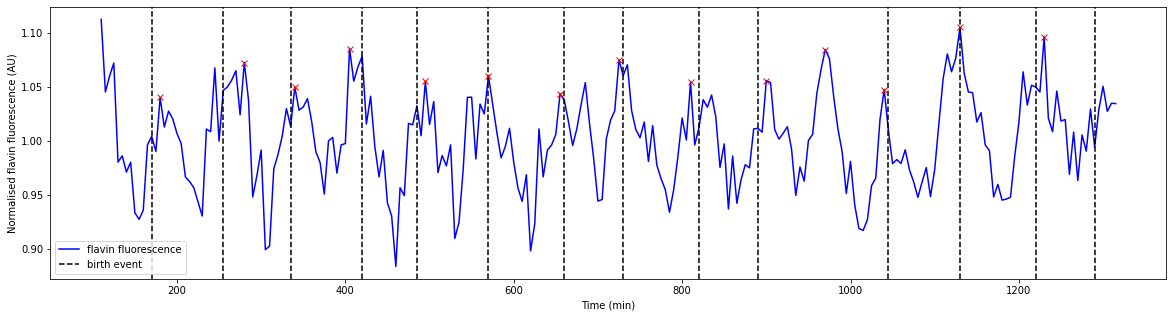
\includegraphics[width=.9\linewidth]{26643_ts.png}
\end{center}

\begin{center}
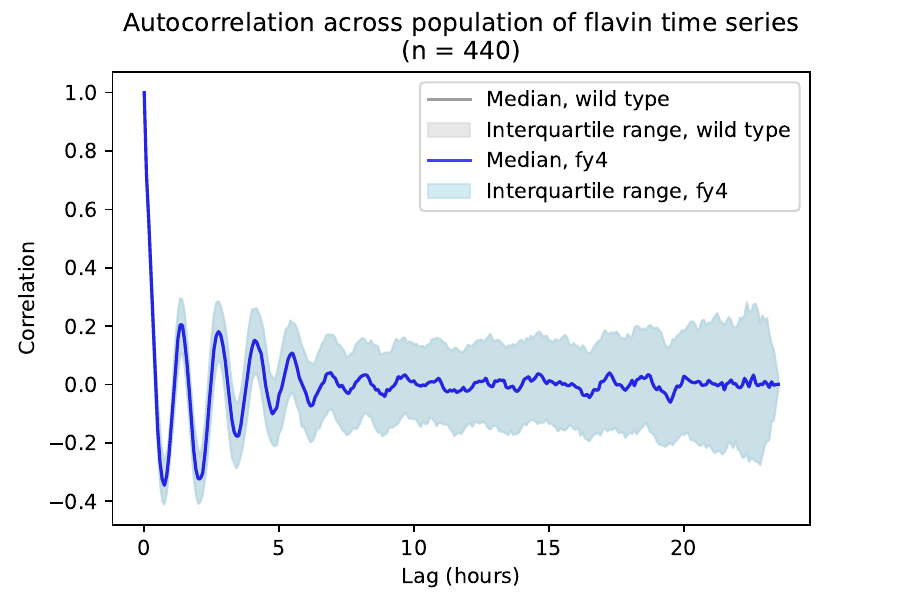
\includegraphics[width=.9\linewidth]{fy4_26643_plots_06.png}
\end{center}
\end{enumerate}

\item Autocorrelation on FitzHugh-Nagumo oscillator
\label{sec:org368123f}

\begin{enumerate}
\item Without noise
\label{sec:orgd112f31}

Generated 400 oscillators with \(RI_{ext}\) = 0.4, \(\tau\) = 12.5, \(a\) = 0.7, \(b\) = 0.82, all out of phase.  This is one of them:

\begin{center}
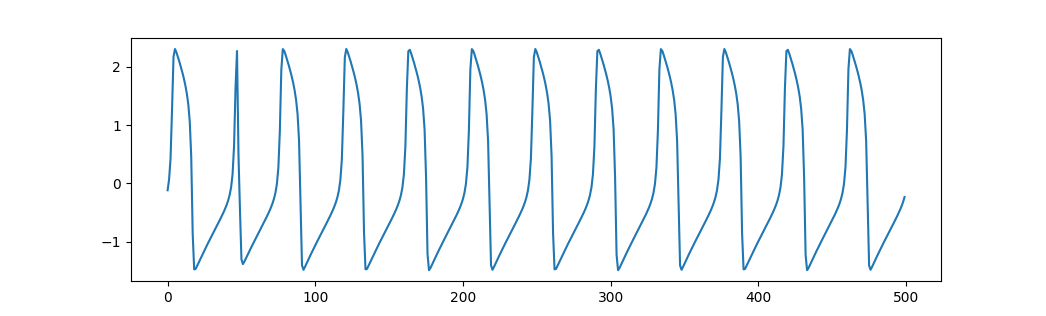
\includegraphics[width=.9\linewidth]{fitzhughnagumo_sample.png}
\end{center}

Autocorrelation function, lag axis scaled by period.  Note slightly different shape of oscillations here compared to sinusoid:

\begin{center}
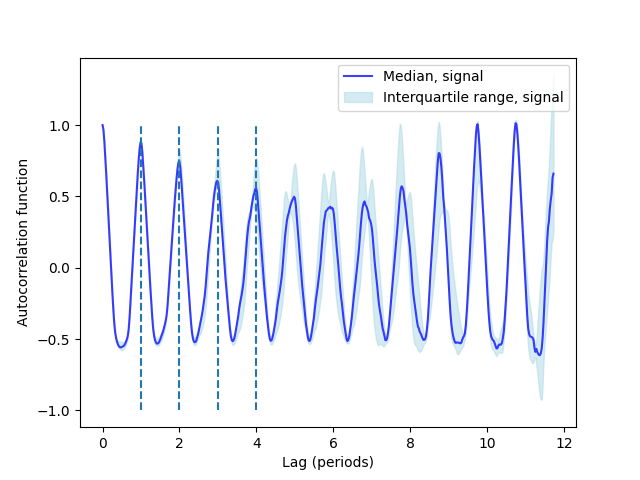
\includegraphics[width=.9\linewidth]{fitzhughnagumo_acf_scalelag.png}
\end{center}

\item With Gaussian noise
\label{sec:orgaa2bb0c}

Sample time series:
\begin{center}
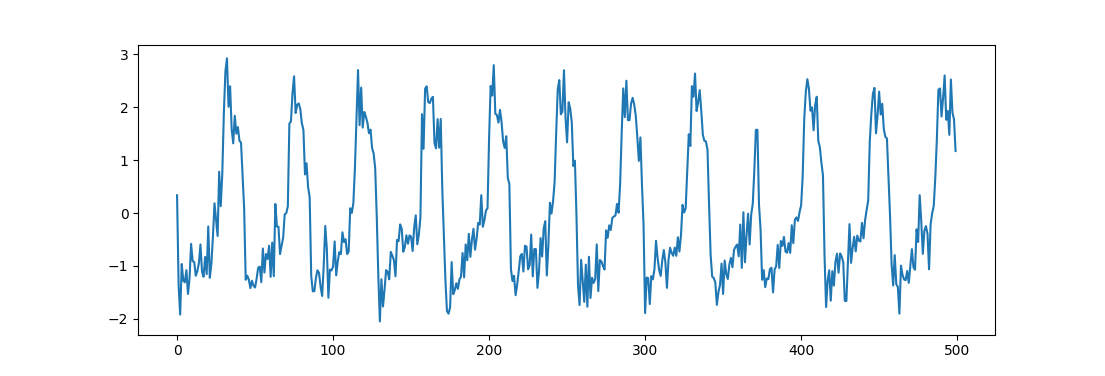
\includegraphics[width=.9\linewidth]{noisyfitzhughnagumo_sample.png}
\end{center}

ACF:
\begin{center}
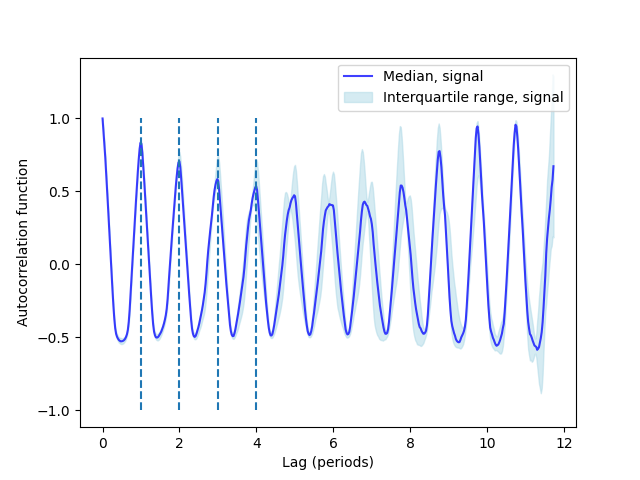
\includegraphics[width=.9\linewidth]{noisyfitzhughnagumo_acf_scalelag.png}
\end{center}

\item With Gillespie noise
\label{sec:org3badb76}

\(k_{0} = 5, d_{0} = 0.05\)

Sample time series: \ldots{}

ACF: \ldots{}

\item Compare with biological oscillator
\label{sec:orga655348}

My intention is to have it model periodic changes in histone 2B intensity levels and yeast cells progress through the cell division cycle.

[FIGURE: some sample time series of FHNs side-by-side with histone 2B oscillations]

\begin{center}
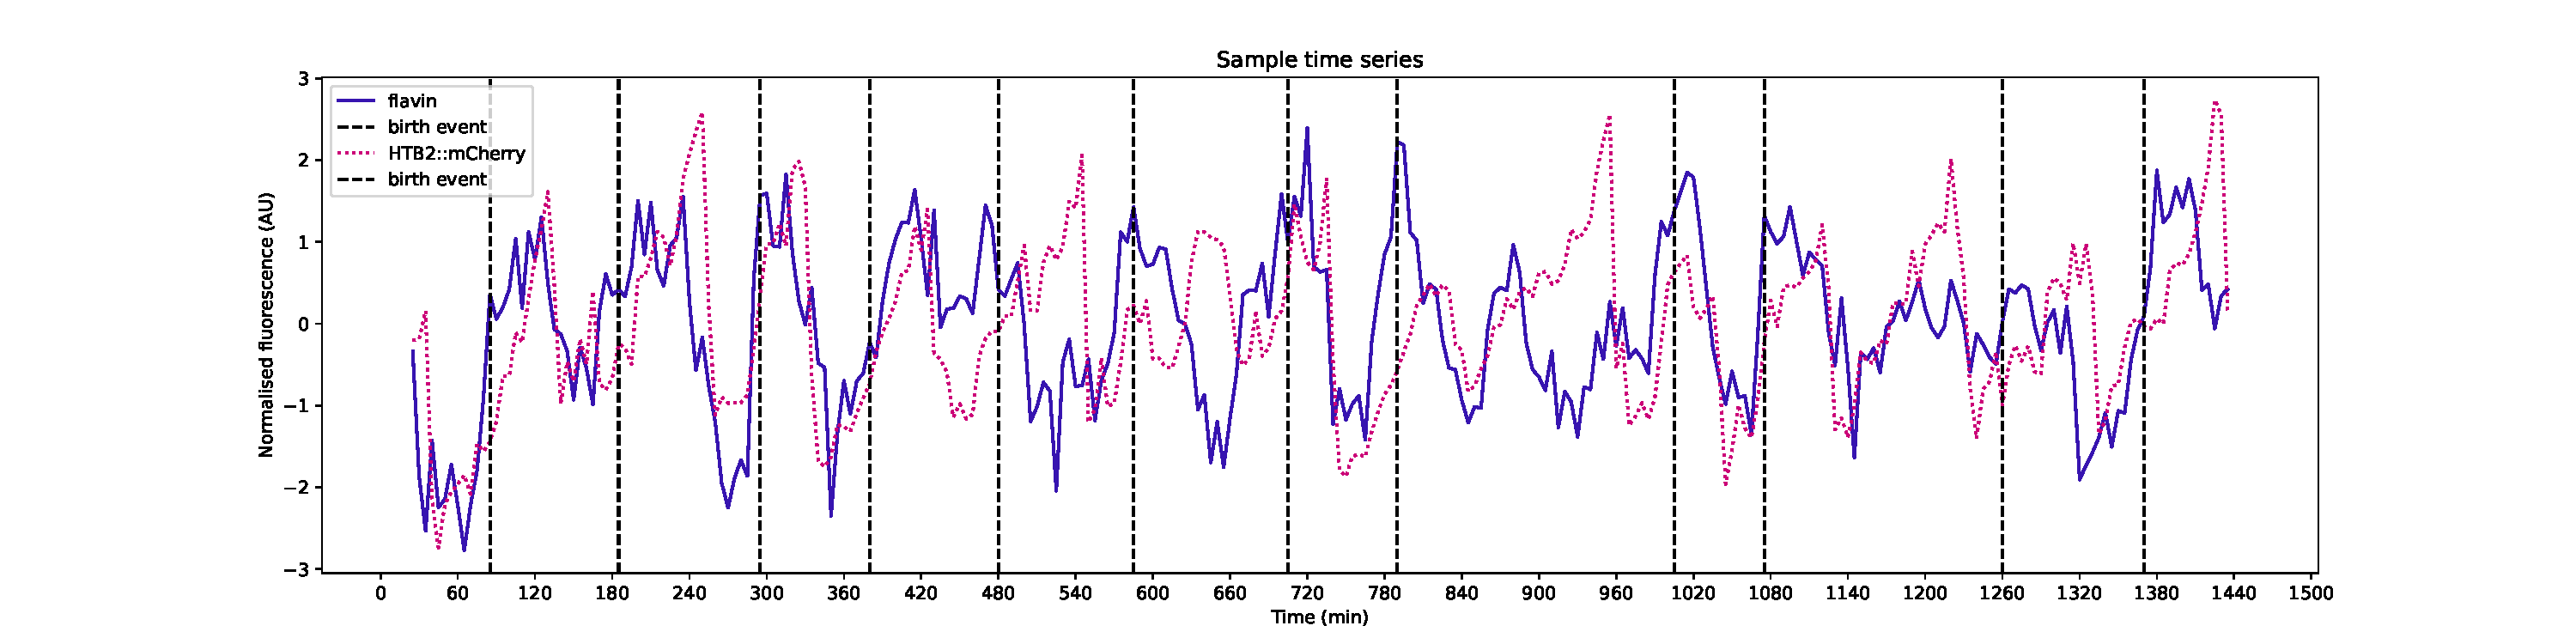
\includegraphics[width=.9\linewidth]{htb2mCherry_26643_plots_purple_01.pdf}
\end{center}

\begin{center}
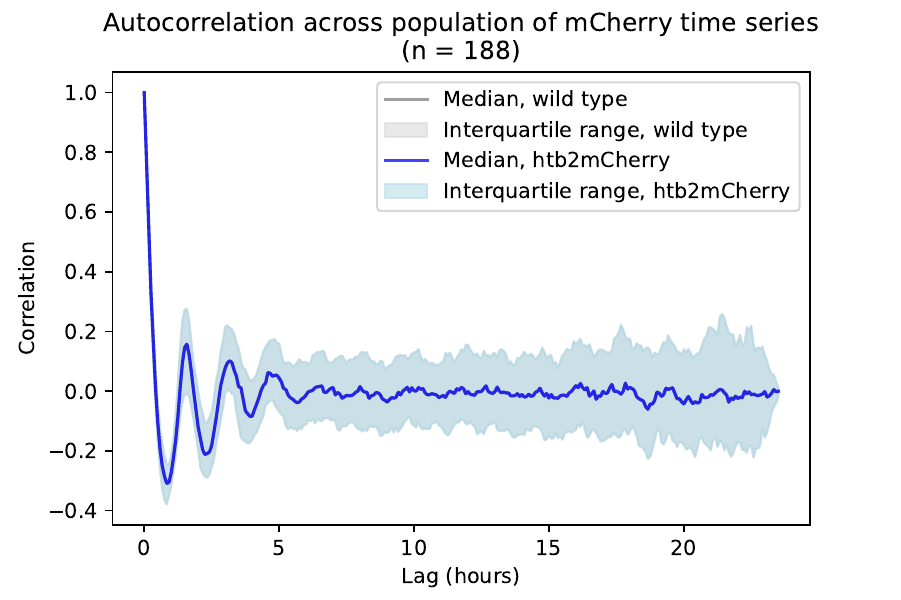
\includegraphics[width=.9\linewidth]{htb2mCherry_26643_plots_mCh_06.png}
\end{center}
\end{enumerate}
\end{enumerate}

% \subsection{Discussion}
% \label{sec:analysis-correlation-discussion}

My investigation aims to address a signal processing question.  Therefore, for the purposes of my investigation, it is not important that these oscillators function as an accurate model of the biological systems responsible for the biological oscillations observed.  Indeed, given that up to 50 flavoproteins may be responsible for flavin autofluorescence, a component of such a poorly biochemically characterised system like the yeast metabolic cycle, it is not feasible to find a mathematical model that accurately describes the biological oscillations.

So long as the time series resemble the real oscillators of interest, the hope is that the conclusions from investigating our simple \& well-characterised models may answer questions on the behaviour and relationships between our real oscillators. [this sentence is a bit vague, but will revisit this after I weave together the story]  Potentially, this investigation can be extended to oscillators modelled by other systems of differential equations that describe other biological rhythms.


\subsection{Combining methods to get a picture of periodicity}
\label{subsec:analysis-characterisation-combined}

As each method comes with own advantages and limitations -- especially apparent when we're dealing with noisy biological data -- it is useful to use several methods in concert get an idea of the periodicity (or other properties) of the oscillations.
For example, \textcite{potvin-trottierSynchronousLongtermOscillations2016} combines the autocorrelation function and the Fourier transform to study the changes in the periodicity of a modified model of the repressilator.
The autocorrelation function, in particular, has been used in the yeast metabolic cycle literature, e.g. \textcite{papagiannakisAutonomousMetabolicOscillations2017}.

Here, I consider combining the autocorrelation function and the Fourier transform, and will use this in my analysis of biological data.

[FIGURE: SHOWS A GOOD TIME SERIES, FFT, ACF, AR, AND THE MOST PROBABLY OSCILLATION FREQUENCY FROM EACH]

[FIGURE: THE SAME AS ABOVE BUT LOOKING AT A POPULATION OF TIME SERIES.  THESE TRAJECTORIES SHOULD HAVE BEEN COMPUTED INDIVIDUALLY FOR EACH TIME SERIES.  THE CAPTION SHOULD EXPLAIN THE MEAN/MEDIAN AND ERROR RANGES.]

\subsection{Revisiting classification to characterise differences between conditions}
\label{subsec:analysis-characterisation-classification_redux}

(This section should be similar to the machine learning section above, but adapted for differences between conditions or strains.)


\section{Clustering: I have many time series (of the same signal) from many cells -- what are their relationships to each other?}
\label{sec:analysis-clustering}

% Literature review subsection
% \subsection{(Literature)}
% \label{subsec:analysis-clustering-literature}

% mini-review -- IT'S PRETTY UNWIELDY AT THIS POINT, AND REFERENCES CONCEPTS NOT DISCUSSED TILL LATER
Clustering of time series has been used to identify groupings within a set of time series \citep{wangStructureBasedStatisticalFeatures2007}, including biological time series \citep{shafieiDopamineSignalingModulates2019}, or even transcript cycling patterns in YMCs \citep{tuLogicYeastMetabolic2005}.
However, \citet{wangStructureBasedStatisticalFeatures2007} and \citet{tuLogicYeastMetabolic2005} employed $k$-means clustering, which requires the user to specify the number of clusters, and therefore may not reflect the underlying structure of the set of time series.
Though \citet{shafieiDopamineSignalingModulates2019} used modularity clustering \citep{newmanModularityCommunityStructure2006}, the method was based on one time series feature, which may not adequately capture the characteristics of the time series.

For my investigation of the yeast metabolic cycle, clustering is important because it can discover structure in a dataset and can summarise the difference between the groups it finds.
And I can also ask the question of whether such differences conform to biological groupings in the dataset -- if so, I can then ask the question of which time series features from each biological grouping is responsible for this.
Furthermore, clustering is important for a dataset from which we expect cell-to-cell heterogeneity.
This thus takes advantage of single-cell microfluidics, as such a platform allows us to study such heterogeneity.

% \subsection{Machine learning approaches to clustering}
% \label{subsec:analysis-clustering-ml}
% - Featurisation -- decisions to make
% - Clustering approaches and algorithms -- compare and contrast
% - Review existing methods first and then talk about the methods I tried, with results.

% Copied from 10m report.
% - Supervised classification is going to be mostly killed because it belongs in a previous section, and I have better data than SM vs SC.
% - Unsupervised clustering: the literature stays, but I'll try doing it on better data.  To add: UMAP.
% ----------------------
\subsection{Graph-based Clustering of Oscillations Based on Feature Vectors}
\label{subsec:analysis-clustering-graphclustering}

Thus, I converted each time series of flavin autofluorescence to a vector of features, and represented the vectors as nodes on a geometric graph.
Such a geometric graph may function as a visualisation tool as well.

% FIGURE: pipeline and options.  It's rather difficult to visualise what happens, so such a figure, like the one I often use in the lab presentations in the summer, will be helpful.  Though may be more impactful in the presentation rather than in this report.

Modularity clustering is the problem of partitioning a graph into clusters in order to optimise a `modularity' value.
This value is defined as the number of edges between clusters minus the number of expected edges if edges are placed at random \citep{newmanModularityCommunityStructure2006}.
The general Louvain algorithm \citep{blondelFastUnfoldingCommunities2008,muchaCommunityStructureTimeDependent2010} is one method to solve this optimisation problem and define partitions for a graph.
This algorithm has a resolution parameter which specifies the scale of the clusters: low resolution gives large clusters, and high resolution gives small clusters \citep{fortunatoResolutionLimitCommunity2007}.

Unsupervised graph-based clustering suggested that the division between complete and minimal media was dominant among time series of flavin autofluorescence. %(figure \ref{fig:EffectofMediaClusters}).
I constructed an incomplete graph to represent the pairwise similarity between time series based on the \emph{catch22} feature vectors.
Then, I identified communities in the resulting network using the general Louvain algorithm.
When the resolution value was set so that the graph was partitioned into two clusters, the clusters conformed well to complete and minimal media groups (figure \ref{fig:EffectofMediaClusters}). % TABLE/NUMBER: Add a 'confusion matrix' (re-use code from 5m) and calculate accuracy (note: revert to some old commit to re-produce this -- why the hell did Fulcher have to change EVERYTHING ughhhhh).  Make clear the point that in each iteration, things are different.
% (this is the where the Rand value can be used instead, but there is no need -- just making a note here).
Such results suggested that unsupervised graph-based clustering may have potential to discover structure in the dataset.

% TODO: REPEAT INVESTIGATION WITH BETTER DATA

\begin{figure}[htbp]
  \centering
  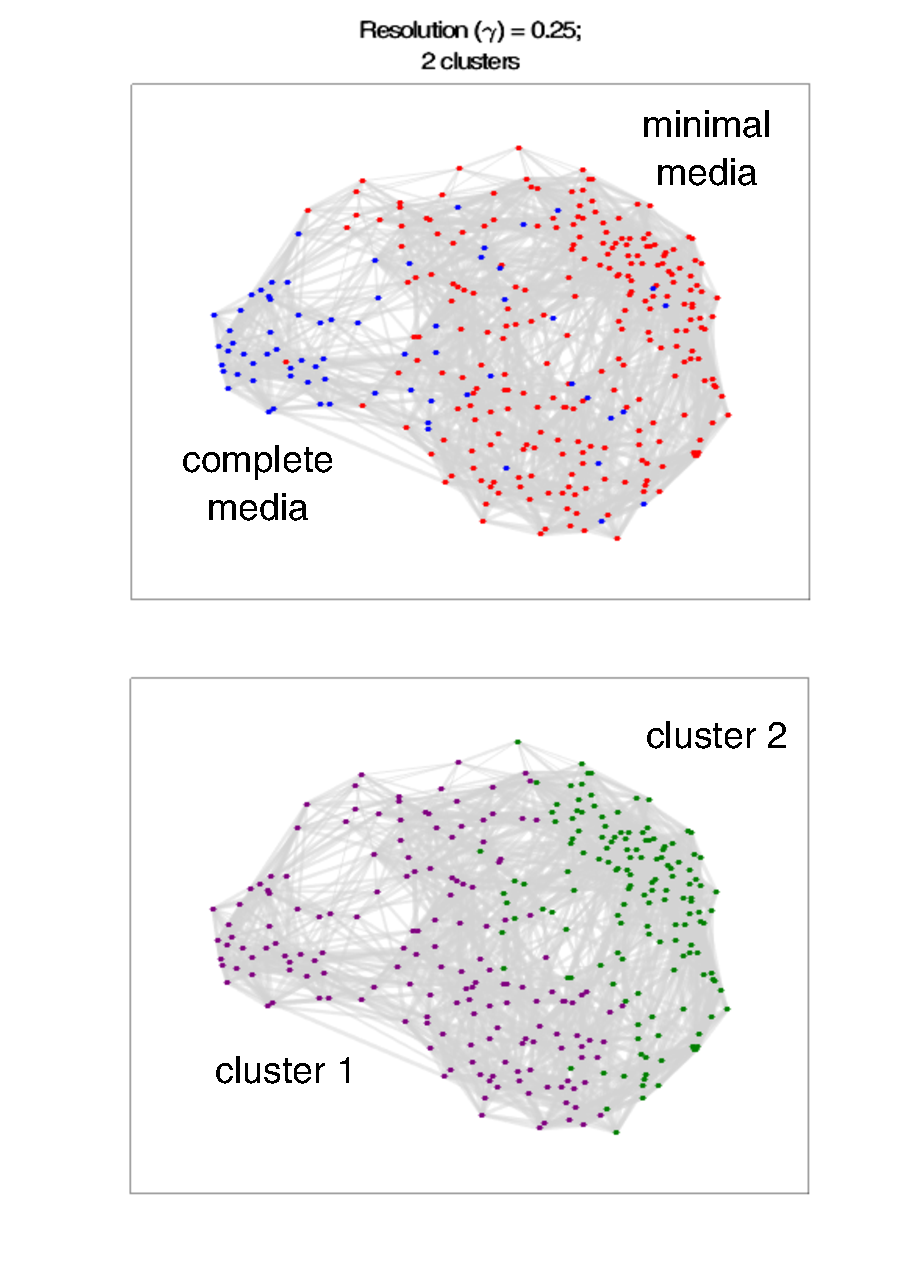
\includegraphics[width=0.5\textwidth]{10m_EffectofMediaClusters}
  \caption{Graph-based clustering partitions a geometric graph defined by pairwise cosine distances between \emph{catch22} vectors close to labels defined by media.}
  \label{fig:EffectofMediaClusters}
\end{figure}

Indeed, I found that the method was able to distinguish time series generated in my project from time series obtained by \citet{baumgartnerFlavinbasedMetabolicCycles2018} (figure \ref{fig:DistanceMatrixBaumgartner}, table \ref{tab:ClusterBaumgartner})
However, this ability to distinguish the data sources may have been because the data from different sources were processed in different ways.

\begin{figure}[htbp]
  \centering
  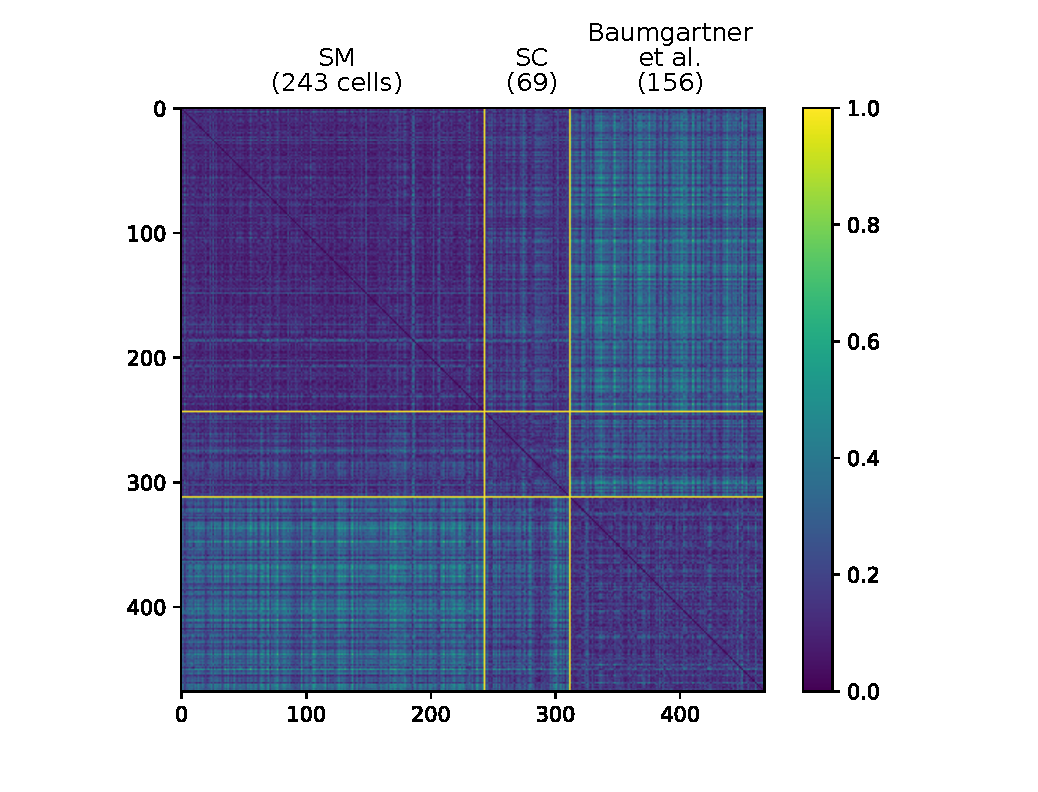
\includegraphics[width=0.6\textwidth]{10m_DistanceMatrixBaumgartner}
  \caption{Graph-based clustering was able to partition minimal media time series, complete media time series, and time series from \citet{baumgartnerFlavinbasedMetabolicCycles2018}.
    This distance matrix is based on cosine distances between \emph{catch22} feature vectors for pairs of time series.  Distances between 0 and 1 (legend, right) are represented as colours.}
  \label{fig:DistanceMatrixBaumgartner}
\end{figure}

\begin{table}[htbp]
  \centering
  \begin{tabular}[h]{rrrr}
    & SM & SC & Baumgartner et al.\\
    Cluster 1 & 1 & 11 & 141\\
    Cluster 2 & 63 & 28 & 6\\
    Cluster 3 & 56 & 22 & 8\\
    Cluster 4 & 79 & 4 & 0\\
    Cluster 5 & 44 & 4 & 1
  \end{tabular}
  \caption{Graph-based clustering is able to partition minimal media time series, complete media time series, and time series from \citet{baumgartnerFlavinbasedMetabolicCycles2018}.  Table shows one graph partition returned by the general Louvain algorithm.  The graph was constructed according to section [METHODS: HCTSA].  In this case, the default value for the resolution parameter was used.}
  \label{tab:ClusterBaumgartner}
\end{table}
% Rand index?

\subsection{Linear techniques}
\label{subsec:analysis-clustering-pca}

(Space for PCA and PCA-initiated t-SNE that I did while doing the UMAP project)

\subsection{UMAP Based on Feature Vectors}
\label{subsec:analysis-clustering-umap}

% TODO: repeat with better datasets
% And it probably saves more time to go over the code again, draft new figures that show my point, and generate new figures, rather than trying to massage the existing figures into this structure.
UMAP \parencite{mcinnesUMAPUniformManifold2020} is a dimension reduction technique that can be used to visualise data, and it preserves the distances between points.
I used UMAP to see if there were intrinsic structures in my datasets, and whether these structures found by such as unsupervised method corresponded to labels, whether oscillatory vs non-oscillatory or labels that distinguish cells from different strains or nutrient conditions.

I used \emph{catch22} as features

% Copied from org note: UMAP to discover structures in flavin datasets

% Notes
% 'labelling custom' refers to using manually-determined oscillatory (0) vs non-oscillatory (1) categories as labels

[FIGURES: 'figures 13-16' from \_resources/umap-figures]

Observations
\begin{itemize}
\item Using labels (strains, oscillation categories) to supervise UMAP works very well.
\item Using catch22 as features doesn't seem to do much better than using raw time points as features.
\item The most interesting plots are figures 13-16:
\begin{itemize}
\item Figure 15 shows that there are two clear clusters of non-oscillatory time series.  This suggests that unsupervised UMAP can discriminate some non-oscillatory time series from the rest.  It's possible that the non-oscillatory time series that cluster with the oscillatory ones may be 'borderline'.  Additionally, comparing this figure with figure 11 shows that using catch22 as features is superior to using time points as features in this context.  The reason these clusters exist in figure 15 and not figure 7 (the equivalent in the other dataset) may be because the BY4741-ZWF1 dataset contains many very high-quality oscillations that are clearly different from the non-oscillatory time series.
\item Comparing figure 15 with figure 13 shows that these non-oscillatory time series are mostly zwf1$\Delta$.  It makes sense because this set of cells have a large group of non-oscillatory flavin signals.
\item Figure 14 shows that there are three clusters among the zwf1$\Delta$ cells, despite supervised UMAP.  Perhaps these have different shapes.  Similarly, figure 16 shows three clusters of non-oscillatory time series; perhaps there are three main non-oscillatory shapes.
\end{itemize}
\end{itemize}

Discussion
\begin{itemize}
\item May need to change the hyperparameters to see if different strains appear in different groups, but it seems to be doing well for some of the plots.
\item Definitely need to visualise the time series associated with each node in the figures; this might reveal the logic behind the structures.  bokeh can be used (see \url{https://umap-learn.readthedocs.io/en/latest/basic\_usage.html}).
\end{itemize}

(Space for discussion according to the figure below.  For example, what can I conclude from this?)

[FIGURE: GRID-SEARCH UMAP PARAMETERS.  THIS FIGURE SHOULD HAVE A 2D GRID OF UMAP PLOTS AS TWO OF THE PARAMETERS ARE VARIED.]

\subsection{Mutual information as similarity for hierarchical clustering}
\label{subsec:analysis-clustering-mi}

\parencite{granadosDistributedDynamicIntracellular2018} describe a mutual information algorithm.

(Copy some of the maths here, explain it a bit)

% TODO: Re-do with better data, better code, etc.
% Or just give up with it because I've shown that mutual information doesn't work so well?
We can see mutual information as a measure for a classification model -- in the same vein as precision, recall, etc.  This is because mutual information produces a value that (indirectly) represents the similarity between two sets of time series data, based on computing confusion matrices via bootstrapping.  To be accurate, mutual information asks the question of to what extent it is possible to distinguish two typical time series sampled from each of two sets of time series.

I can then compute the mutual information between pairs of strains in a dataset, then use the mutual information as a distance measure to produce hierarchical clustering between the strains.

I divide this into three cases:
\begin{enumerate}
\item Include oscillatory time series only.
\item Include non-oscillatory time series only.
\item Include all time series.
\end{enumerate}

Unless otherwise noted, I restrict the range (time points 25 - 168), detrend using a sliding window of 45 time points, and featurise using catch22.  Scaling the features is already included in the mutual information code, and thus not repeated before.  With the mutual information code, I use 1000 bootstraps.

\subsubsection{Causton strains (19979)}
\label{sec:org14969a0}

This is the older experiment with the defective CEN.PK strain but with more cells in total.

Oscillatory only
\label{sec:org468bf6f}

Distance matrix

\begin{center}
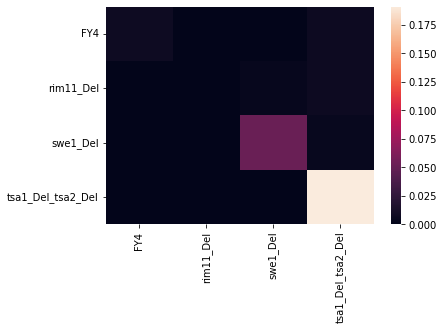
\includegraphics[width=.9\linewidth]{MIHierClust_19979_osc_distmatrix.png}
\end{center}

Dendrogram (UPGMA)

\begin{center}
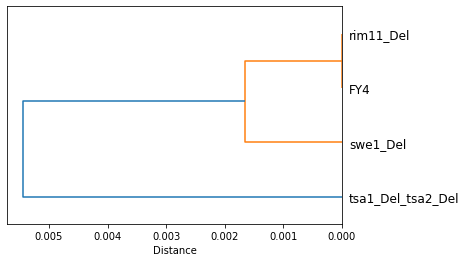
\includegraphics[width=.9\linewidth]{MIHierClust_19979_osc_dendrogram.png}
\end{center}

This suggests that the Causton strains' time traces are very similar to each other.

Switching to using time series as features did not change the values by much -- they were still zero or near-zero.

Non-oscillatory only
\label{sec:org0984c97}

Distance matrix

\begin{center}
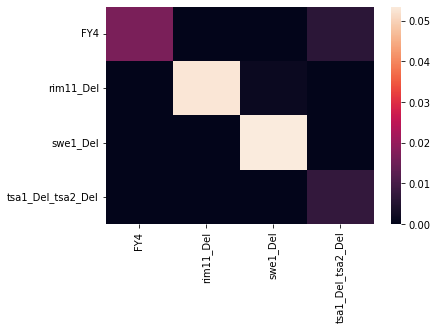
\includegraphics[width=.9\linewidth]{MIHierClust_19979_nosc_distmatrix.png}
\end{center}

Dendrogram (UPGMA)

\begin{center}
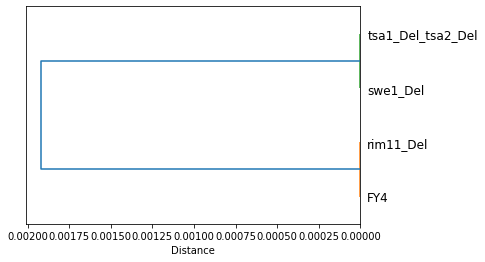
\includegraphics[width=.9\linewidth]{MIHierClust_19979_nosc_dendrogram.png}
\end{center}

This suggests that non-oscillatory time series are similar between strains, which justifies removing them from the feature matrix when performing UMAP in (Identifying the most important catch22 features for classification).  Additionally, removing non-oscillatory time series make biological sense -- we want to see whether single-cell flavin oscillations differ between the strains, and it doesn't make sense to have non-oscillatory time series from potentially dead cells, technical issues, or noise in the data.

All cells
\label{sec:org0854ace}

Distance matrix

\begin{center}
\includegraphics[width=.9\linewidth]{MIHierClust_19979_all_distmatrix.png}
\end{center}

Dendrogram (UPGMA)

\begin{center}
\includegraphics[width=.9\linewidth]{MIHierClust_19979_all_dendrogram.png}
\end{center}

The small distances when all cells are included further justifies the removal of non-oscillatory time series.

\subsubsection{Causton strains (20212)}
\label{sec:orgcc0d5be}

This is the newer experiment with the correct CEN.PK strain from Peter Kötter, but fewer cells in total.

Oscillatory only
\label{sec:org803a4be}

Distance matrix

\begin{center}
\includegraphics[width=.9\linewidth]{MIHierClust_20212_osc_distmatrix.png}
\end{center}

Dendrogram (UPGMA)

\begin{center}
\includegraphics[width=.9\linewidth]{MIHierClust_20212_osc_dendrogram.png}
\end{center}

Same story, we can't tell the strains apart.

\subsubsection{BY4741 vs zwf1$\Delta$}
\label{sec:org7a4d63f}

Oscillatory only
\label{sec:org3fdb03d}

Distance matrix

\begin{center}
\includegraphics[width=.9\linewidth]{MIHierClust_20016_osc_distmatrix.png}
\end{center}

This suggests that there is a considerable difference between these two strains.  Given how classifiers tend to be able to tell apart these strains very well, it is not surprising.

Switching to using time series as features gives a median MI of 0.46 (median 0.46368494, IQR 0.40093307 -- 0.51805235), which isn't a big change from before.

\subsubsection{Remarks}
\label{sec:orga7cc61d}

\begin{itemize}
\item MI with itself: some cases are non-zero (or, not close to zero).  Does this mean that there is enough variety within the dataset concerned that there is a risk of overfitting?
\item This is probably an additional line of evidence to confirm that there is no real difference between Causton strains in terms of their single-cell flavin oscillations.
\item Potential extension: to wild-type/prototrophic strains in different glucose concentrations.
\end{itemize}


\section{Correlation: I have two signals from the same cell -- what are their relationships to each other?}
\label{sec:analysis-correlation}

So far, we have only considered one type of time series from the yeast metabolic oscillator -- the flavin signal.
However, the yeast metabolic oscillator and the cell division cycle form part of a system of coupled oscillator; certainly, in my experiments I record signals that monitor both.
Investigating correlations between two paired time series, originating from the same cell, leads to an understanding of the relationship between the two oscillators.
The most important being the phase relationship: does one oscillation lag behind the other, to what extent, and is this consistent across cells?

\subsection{Cross-correlation}
\label{sec:analysis-correlation-xcf}

Cross-correlation, widely used in signal processing, is used to measure how similar two time series are as the displacement of one relative to the other is shifted across the length of the time series.
To put it in the context of autocorrelation discussed earlier, autocorrelation is a special case of cross-correlation in which the two signals are identical.
In mathematical terms, cross-correlation is defined as:

[INSERT EQUATIONS HERE]

In a biological context, cross-correlation has been used to investigate how fluctuations in transcription levels influence fluctuations in protein expression in \emph{E. coli} [CHECK CITATION AGAIN TO VERIFY IF TRUE] \parencite{dunlopRegulatoryActivityRevealed2008},
and to investigate the relationship between instantaneous growth rate and the expression of \emph{lac} genes OR of enzymes in central metabolism across a population of \emph{E. coli} cells \parencite{kivietStochasticityMetabolismGrowth2014}.
Importantly, these studies are derived from single-cell microfluidics experiments with time-lapse microscopy, and therefore their treatment of a population of time series is useful for my case.

Therefore, my use of cross-correlation is adapted from theirs so that it suits a population of time series, which is the thing that I have.

[INSERT EQUATIONS HERE]

As I did for my discussion of autocorrelation, I will start with the sinusoid and FitzHugh-Nagumo oscillators as simulations of my biological time series to show understanding of the methods,
then move on to an example of a real dataset.

% - Cross-correlation: start from the basic definitions, then extend to population-level cross-correlation as used by Kiviet et al. (2014)

% Copied from project: 'Modelling cross-correlation between sinusoids and relaxation oscillators',
% or, my 'synthetic oscillations report'.
% Currently doesn't really fit the thesis so much -- it comes with its own subsections, and this part can definitely be shorter.  Certainly, there shouldn't be a 'results' subsection.

% (some text used to be here)

\begin{enumerate}
\item Cross-correlation between harmonic and FitzHugh-Nagumo oscillators
\label{sec:orgd5cc0d1}

\begin{enumerate}
\item Without noise
\label{sec:org2f425b6}

Original time series
\begin{center}
\includegraphics[width=.9\linewidth]{sinusoid_and_fitzhughnagumo_nonoise.png}
\end{center}

Cross-correlation function, 400 signal pairs (each signal pair randomly phase-shifted)
\begin{center}
\includegraphics[width=.9\linewidth]{randomshift_sinusoid_fitzhughnagumo_xcf.png}
\end{center}

Shift of this function from the origin indicates the lag of one time series with respect to another.  This is the point of using cross-correlation, i.e. quantifying this lag across a population of time series.

\item With Gaussian noise
\label{sec:org8b120ec}

Original time series
\begin{center}
\includegraphics[width=.9\linewidth]{sinusoid_and_fitzhughnagumo.png}
\end{center}

Cross-correlation function (each signal pair randomly phase-shifted)
\begin{center}
\includegraphics[width=.9\linewidth]{randomshift_sinusoid_fitzhughnagumo_noisy_xcf.png}
\end{center}

\item Compare with biological oscillator
\label{sec:orgeeca8c5}

Cross-correlation function between flavin autofluorescence oscillations and histone 2B levels, across a population of cells:

\begin{center}
\includegraphics[width=.9\linewidth]{xcf.pdf}
\end{center}
\end{enumerate}
\end{enumerate}

\subsection{Granger Causality}
\label{sec:analysis-correlation-granger}

Granger causality is another method of assessing the relationship between two time series.
It is a statistical hypothesis test used to answer the question of whether one time series is useful for predicting another [CITATION FOR GRANGER CAUSALITY TEST NEEDED] -- in other words, it evaluates precedence of one time series relative to another.
The logic of the Granger causality test is that: given a time series X and a time series Y, if you can predict values of Y based on the values of X better than you can predict values of Y based on the past values of Y, then X Granger-causes Y.
This method is used a lot in econometrics and climate science [CITATIONS NEEDED].
[AND DO BIOLOGISTS USE IT?]

(Add content when I figure out how to make this investigation work.)

\section{Summary}
\label{sec:analysis-summary}
% - Justification of each steps of my pipeline

% I expect this will be improved when I go through the whole analysis again and get good take-home messages in my head.
I've described the way that I process my single-cell time series data, broken down into five main steps: cleaning data, classification of oscillatory time series, characterisation of features of oscillatory time series, clustering of similar time series in a large dataset, and correlation of two related time series.
This can form an analysis workflow which can be adapted to other biological rhythms or analysis of large datasets of time series in general.
And this can be an interesting software engineering question to bring it all together.

In each step of the way, there are several methods to choose from, each with its own merits and caveats -- mostly because there doesn't seem to be an agreed-upon standardised way to solve problems.
This is particularly highlighted in the many `judgement calls'.
In cleaning data, the analyst must decide on a threshold to filter out useless data from the useful ones, but without compromising on the size of the resulting dataset so the remaining dataset is still useful.
In classification of oscillatory time series: rhythmicity detection inevitably hinges upon defining a threshold between `oscillatory' and `non-oscillatory'.
Furthermore, it is difficult to do this with noisy and relatively short (on the order of 10 oscillations, rather than 1000) time series.
Characterisation of oscillatory time series is more `objective', but there are issues in the representation of properties like shape and phase.
And the machine learning methods rely on supplying a training set, choosing appropriate featurisation methods, and tuning hyperparameters, as with any other machine learning method.

Solving mathematical and computational problems for each task is an intellectual investigation in its own right (each can spin off to form its own thesis), and opens more questions than answers.
And so future directions include things like using Bayesian method to classify oscillations, or whether better data or better featurisation helps.

I illustrate the use of my analysis workflow in the next chapter, when I apply it to biological results.
